\documentclass[10pt,aspectratio=169]{beamer}

\usetheme[progressbar=frametitle]{metropolis}

\title{Mathematical Foundations of Computer Science}
\subtitle{Decidability of String Graphs}
\date{26.01.2023}
\author{Pavel Zwerschke}
\institute{Radboud University Nijmegen}
\titlegraphic{\hfill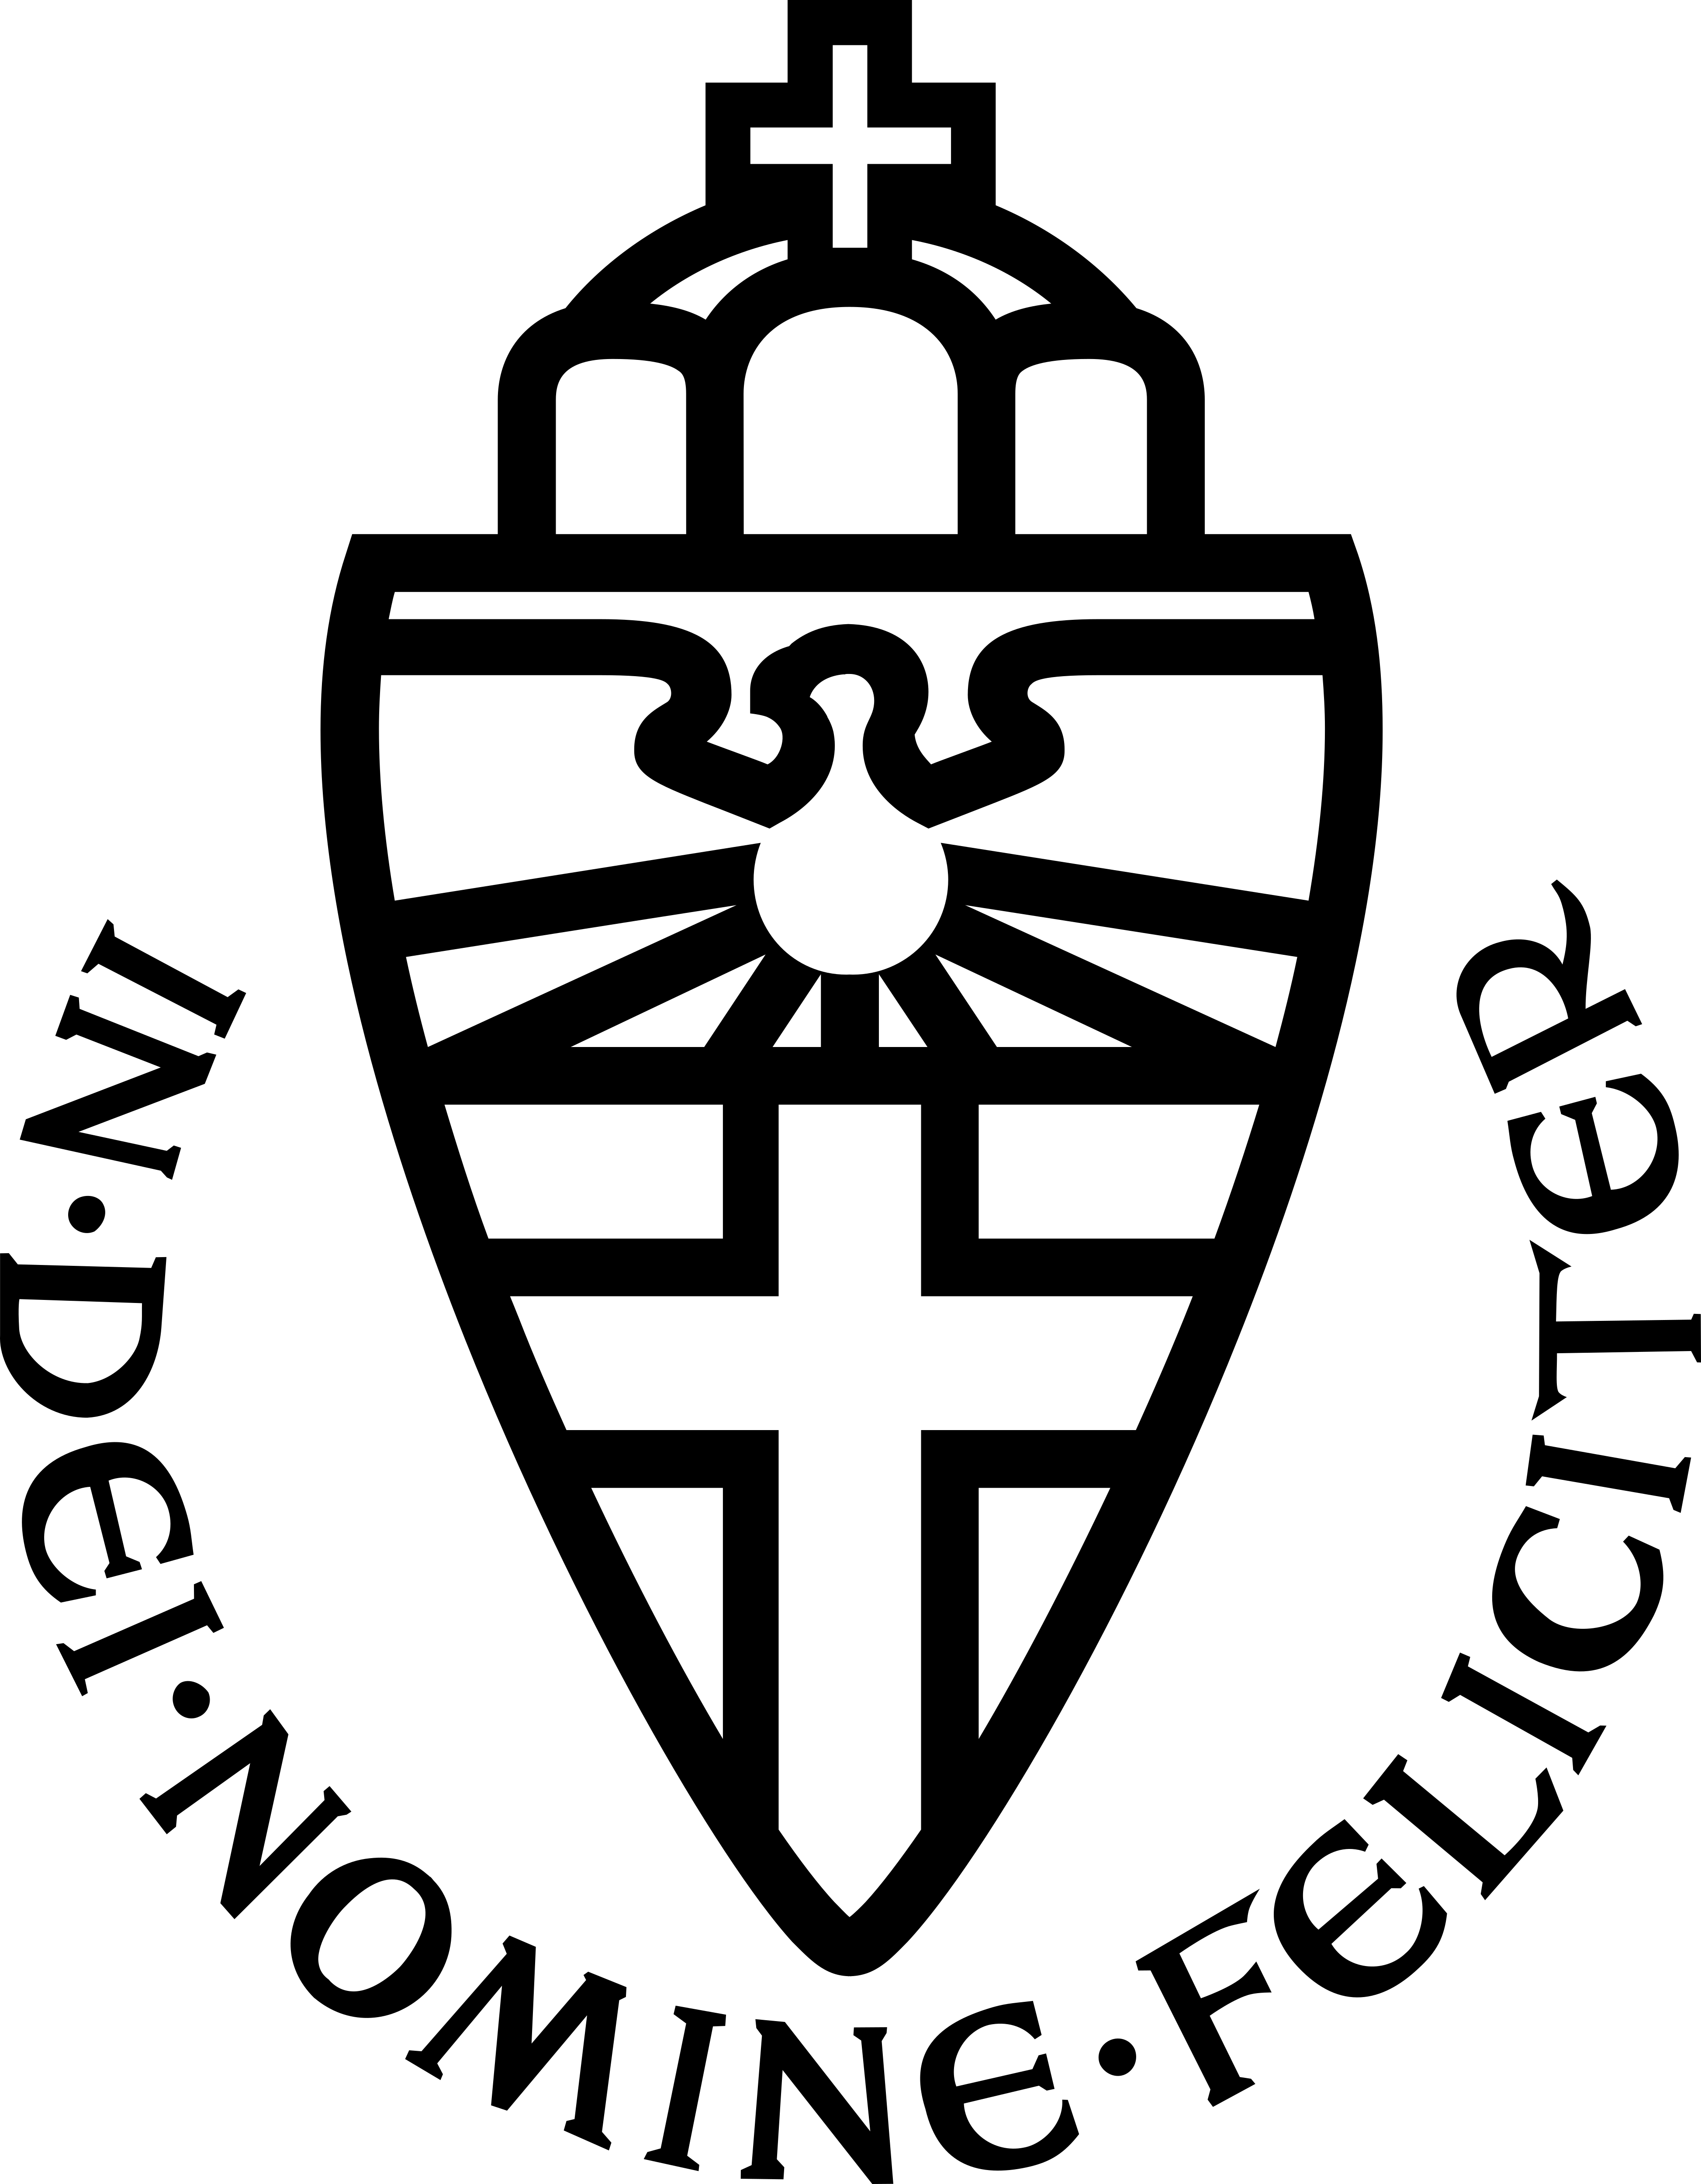
\includegraphics[height=1.5cm]{logos/radboud-university}}

% BibTeX setup
\usepackage[backend=bibtex, bibstyle=alphabetic, citestyle=alphabetic]{biblatex}
\bibliography{references}

\usepackage[english]{babel} % English

\usepackage{amsmath}
\usepackage{amssymb}
\usepackage{amsthm}
\usepackage{mathtools}
\usepackage{xcolor}

\definecolor{highlight}{RGB}{255, 136, 213}

\usepackage{graphicx}

\theoremstyle{plain}

\setbeamertemplate{theorems}[numbered]
\newtheorem*{lemma*}{Lemma}

\newcommand{\N}{\mathbb{N}}
\newcommand{\R}{\mathbb{R}}
\newcommand{\Z}{\mathbb{Z}}

\newcommand{\set}[1]{\{#1\}}

\begin{document}

\maketitle

\section{Introduction}

\begin{frame}{What is a string graph? \cite{schaefer01}}
    \setbeamertemplate{background}[grid]
    \begin{itemize}
        \item A \textit{curve} (or \textit{string}) is a set homeomorphic to \([0,1]\)
        \item Given a collection of curves \((C_i)_{i \in I}\) in the plane, the corresponding intersection graph is \( (I, \set{\set{i, j} : C_i \text{ and } C_j \text{ intersect}}) \)
        \item \textit{string graph}: a graph isomorphic to the intersection graph of a collection of curves 
    \end{itemize}
\end{frame}

\begin{frame}{Non-string graph example \cite{sinden66}}
    There are graph instances that cannot be string graphs.

    \begin{center}
        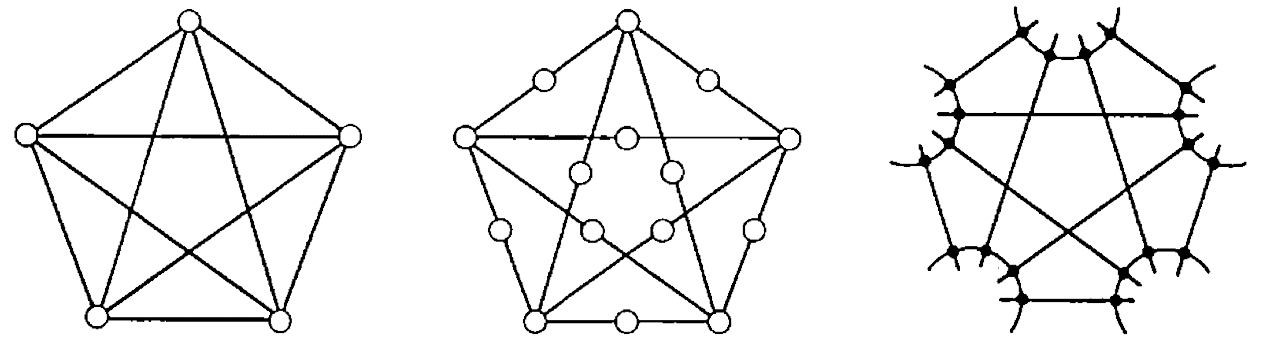
\includegraphics[width=0.8\textwidth]{images/figure-0.png}
    \end{center}
\end{frame}

\begin{frame}{Definitions}
    \begin{itemize}
        \item \textit{size} of a collection of curves: the number of intersection points
        \item \(c_s(G)\): the size of the smallest (smallest number of intersections) set of curves whose intersection graph is isomorphic to \(G\)
        \item Define \(c_s(m) = \max\set{c_s(G) : G \text{ has } m \text{ edges}}\)
    \end{itemize}
\end{frame}

\begin{frame}{\(c_s(G)\) is finite \cite{schaefer01}}
    \begin{itemize}
        \item It is not obvious that \(c_s(G)\) is finite for every string graph \(G\)
        \item Kratochvíl et al. showed that \(c_s(G)\) is finite for every string graph \(G\)
    \end{itemize}
    \begin{lemma}
        A string graph can be realized by a family of polygonal arcs with a finite number of intersections.
        \label{lem:finite-cs}
    \end{lemma}
\end{frame}

\addtocounter{theorem}{-1}
\begin{frame}[t]{Lemma \ref{lem:finite-cs} Proof}
    \begin{lemma}
        A string graph can be realized by a family of polygonal arcs with a finite number of intersections.
    \end{lemma}
    \begin{columns}
        \begin{column}{0.5\textwidth}
            \begin{itemize}
                \item Let \((C_i)_{i\in I}\) be a family of curves in the plane.
                \item<2-> Let \(C \coloneqq \bigcup_{i\in I}C_i\). \(C\) is compact (bounded and closed).
                \item<3-> For \(p \in C\) find an open neighborhood \(O_p\) of \(p\) such that \(C \cap O_p\) is only on one curve (or two if they intersect in \(p\)).
                \item<4-> \(\mathcal{O} \coloneqq \set{O_p : p \in C}\) is an open cover of \(C\).
                \item<5-> \(\mathcal{O}\) can be refined to a finite subcover \(\mathcal{O}'\).
                \item<6-> In each \(O \in \mathcal{O}'\), replace the curves by polygonal arcs. \qed
            \end{itemize}
        \end{column}
        \begin{column}{0.5\textwidth}
            \includegraphics<1-2>[width=\textwidth]{images/figure-18.pdf}%
            \includegraphics<3>[width=\textwidth]{images/figure-19.pdf}%
            \includegraphics<4>[width=\textwidth]{images/figure-20.pdf}%
            \includegraphics<5>[width=\textwidth]{images/figure-21.pdf}%
            \includegraphics<6->[width=\textwidth]{images/figure-22.pdf}%
        \end{column}
    \end{columns}
\end{frame}

\begin{frame}{Realizability}
    \begin{itemize}
        \item Graph \(G = (V, E)\), \(R \subseteq \binom{E}{2} = \set{\set{e, f} : e, f \in E} \) on \(E\)
        \item call a drawing \(D\) of \(G\) in the plane a \textit{weak realization} of \((G, R)\) if only pairs of edges \(\in R\) are allowed to intersect in \(D\)
        \item call a drawing \(D\) of \(G\) in the plane a \textit{realization} of \((G, R)\) if exactly pairs of edges \(\in R\) are intersect in \(D\)
        \pause
        \item \(c_w(G, R)\) is the smallest number of intersections in a weak realization of \((G, R)\)
        \item \(c_w(G) = \max\set{c_w(G, R) : (G, R) \text{ has a weak realization}} \)
        \item \(c_w(m) = \max\set{c_w(G) : G \text{ has } m \text{ edges}}\)
        \item Define \(c_r(G, R)\), \(c_r(G)\) and \(c_r(m)\) similarly for realizations
        \pause
        \item \(\mathrm{cr}(G) = c_w(G, \binom{E}{2})\) is known as the crossing number (\(\mathbf{NP}\)-complete)
        \item \(c_w(G, \emptyset)\) is equivalent to planarity testing (in \(\mathbf{P}\))
    \end{itemize}
\end{frame}

\begin{frame}{Relationships between realizability functions \cite{schaefer01} \cite{kra91b}}
    \begin{lemma}
        \(c_r\), \(c_w\) and \(c_s\) are equivalent in the following sense:
        \begin{itemize}
            \item \(c_w(m) \leq c_r(m)\)
            \item \(c_r(m) \leq 4 c_s(m^2 + 4m)\)
            \item \(c_s(m) \leq 4 c_w(2m) + 2m\)
        \end{itemize}
        \label{lem:pol-equivalent}
    \end{lemma}
\end{frame}

\begin{frame}{\textsc{Realizability} \(\propto\) \textsc{String}}
    Let \(G = (V, E)\), \(R \subseteq \binom{E}{2}\) be a realizability problem. \pause
    Construct \(V' = V \cup E \cup \set{(u, e) : u \in e \in E}\) 
    and \(E' = R \cup \set{ \set{u, (u,e)}, u \in e \in E} \cup \set{\set{e, (u,e)}, u\in e \in E}\). \pause
    Then \((G, R)\) is realizable iff \(G' = (V', E')\) is a string graph.
    \begin{center}
        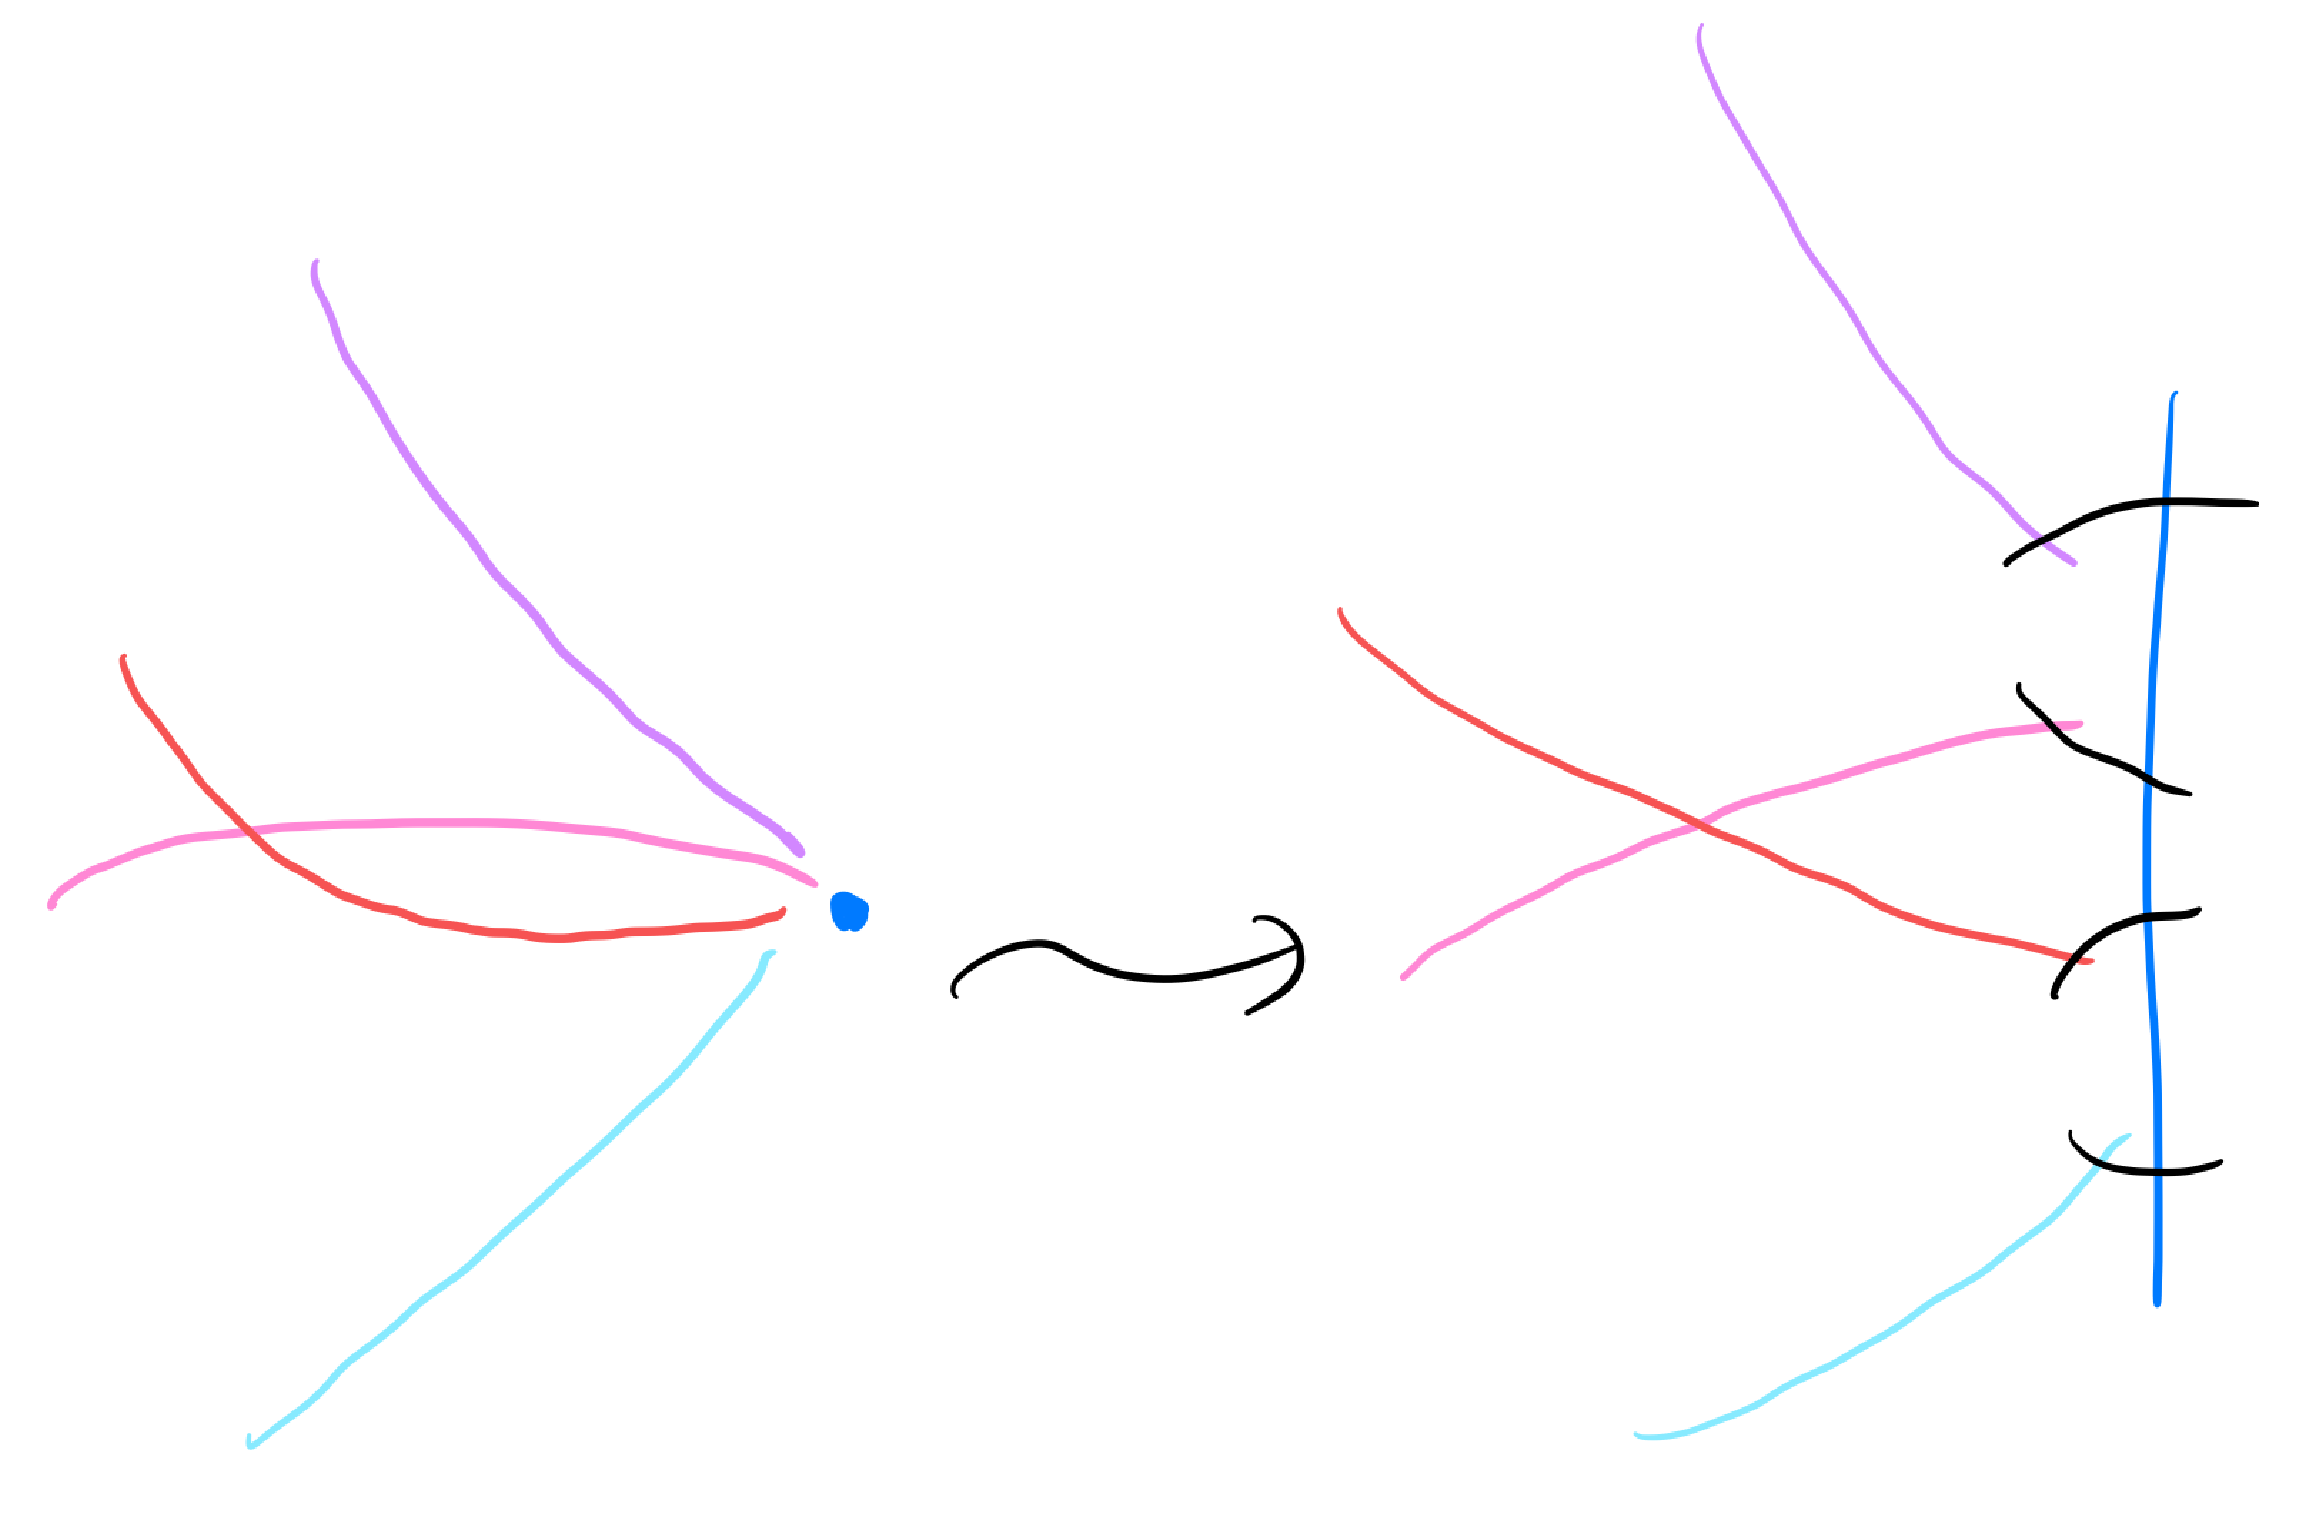
\includegraphics[height=0.5\textheight]{images/figure-2.pdf}
    \end{center}
\end{frame}

\begin{frame}{\textsc{String} \(\propto\) \textsc{Weak Realizability}}
    Let \(G = (V,E)\) be a string graph instance. \pause
    Define the following problem \((G', R)\):\\
    \(G' = (V \cup E, \set{\set{u,e} : u \in e \in E})\) and\\
    \(R = \set{\set{\set{u,e}, \set{v,f}} : \set{u,v} \in E}\).
    \begin{center}
        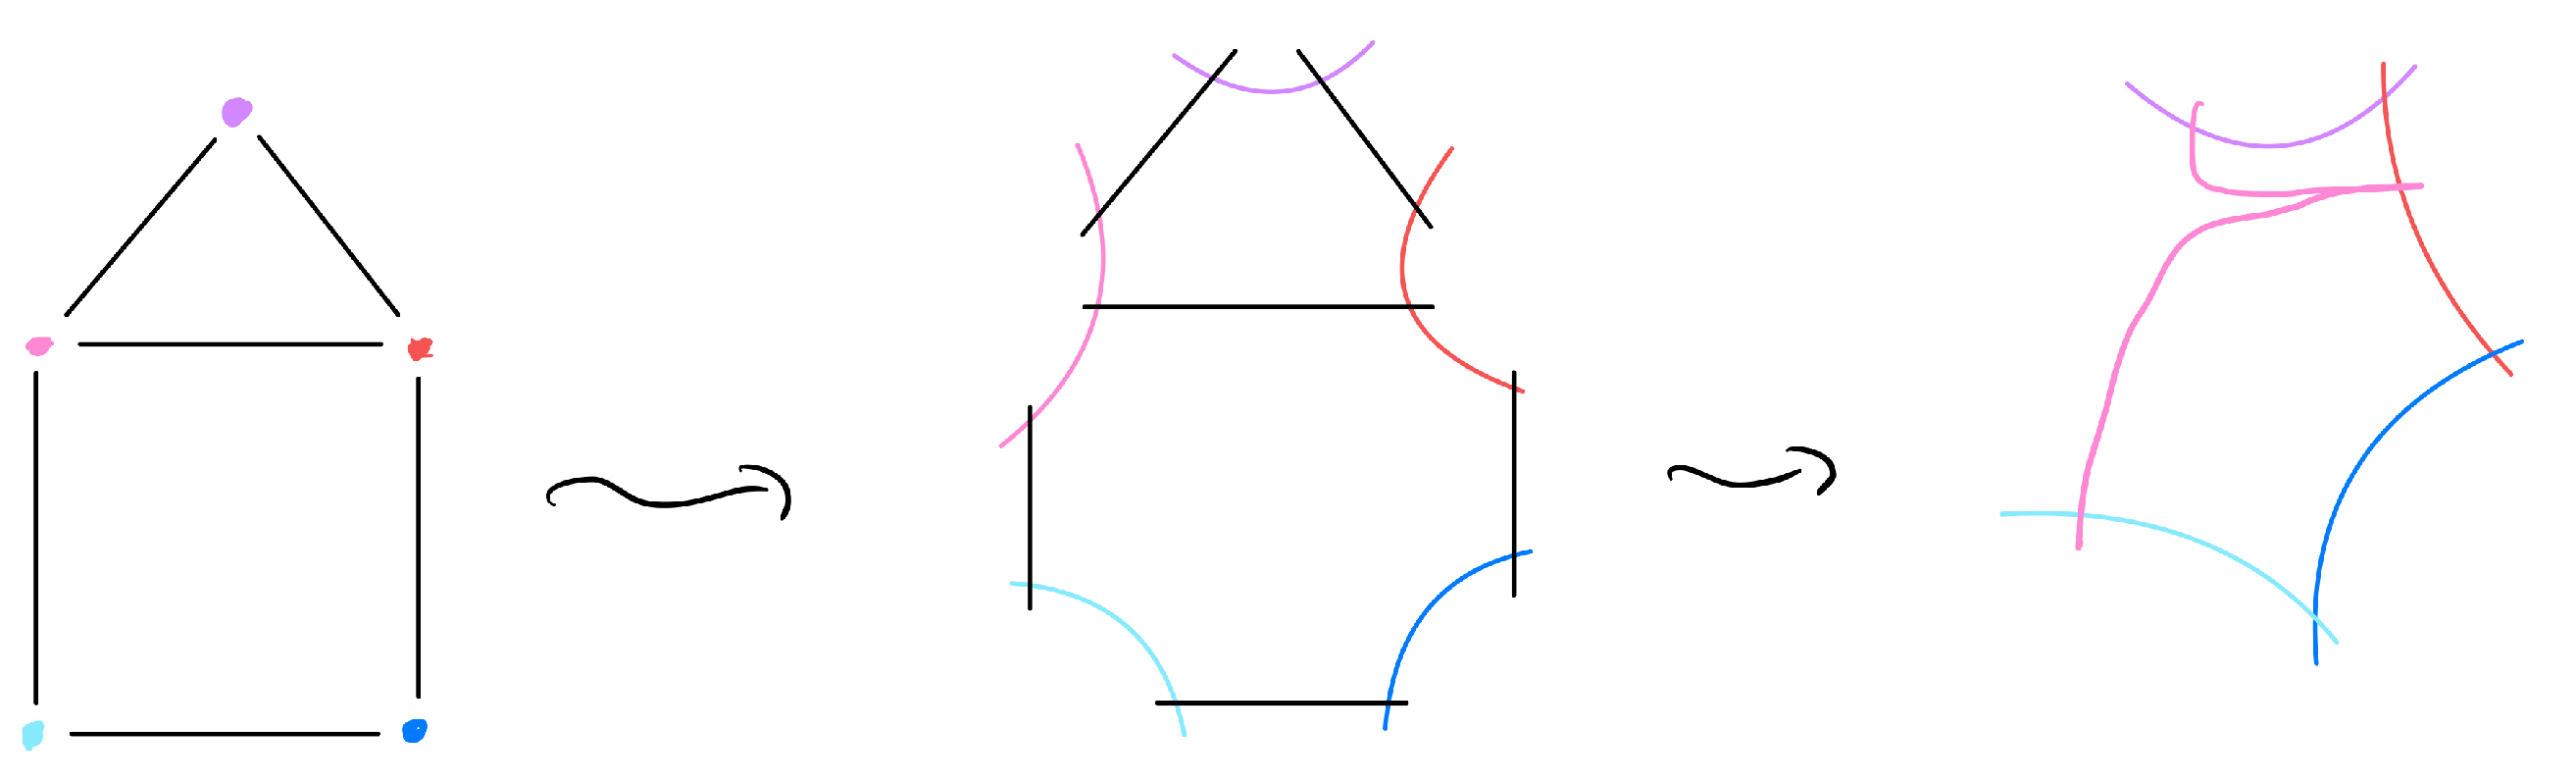
\includegraphics[height=0.4\textheight]{images/figure-3.pdf}
    \end{center}
\end{frame}

\section{Bounding the Number of Intersections \cite{schaefer01}}

\begin{frame}{Bounding the Number of Intersections -- Strategy}
    Show by contradiction: There exists a drawing for a realizability problem 
    s.t. there are \(< 2^m\) intersections for each edge \(e\) in \(D\).\pause

    This gets translated into a string graph problem with Lemma \ref{lem:pol-equivalent}.\pause

    Every string graph must have a representation with maximally exponential size.\pause

    Construct an algorithm to check if something is a string graph in \(\mathbf{NEXP}\).
\end{frame}

\begin{frame}{Bounding the Number of Intersections 1}
    \begin{lemma}
        Every word of length \(\geq 2^n\) over an alphabet of size \(n\) contains a non-trivial (contiguous) subword in which every character occurs an even number of times.
        \label{lem:even-occurrences}
    \end{lemma}
\end{frame}

\addtocounter{theorem}{-1}
\begin{frame}[t]{Lemma \ref{lem:even-occurrences} Proof}
    \begin{lemma}
        Every word of length \(\geq 2^n\) over an alphabet of size \(n\) contains a non-trivial (contiguous) subword in which every character occurs an even number of times.
    \end{lemma}
    \begin{columns}
        \begin{column}{0.4\textwidth}
            \begin{itemize}
                \item Let \(\Sigma = \set{1, \ldots, n}\), \(w \in \Sigma^*, |w| \geq 2^n\).
                \item<2-> \(\forall i \in \set{0, \ldots, 2^n}\), assign a vector \(v_i \in \Z_2^n\) whose \(j\)-th coordinate \(=\) parity of \#occurences of symbol \(j\) in the \(w[:i]\).
                \item<6-> \(\exists 2^n + 1\) indices \(\Rightarrow\) Pigeonhole Principle \(\Rightarrow\) \(\exists i < j\) with \(v_i = v_j\).
                \item<7-> For \(w' \coloneqq w[(i+1):j]\), every symbol occurs an even number of times. \qed
            \end{itemize}
        \end{column}
        \begin{column}{0.6\textwidth}
            \textbf{Example:}
            \(w = {\color<3-4>{highlight}1}{\color<4>{highlight}2}312231, |w| = 8 \geq 2^3\)\pause

            \[ v_0 = \begin{pmatrix}
            0 \\ 0 \\ 0
            \end{pmatrix}\pause{}, v_1 = \begin{pmatrix}
            1 \\ 0 \\ 0
            \end{pmatrix}\pause{},
            {\color<6->{highlight} v_2 = \begin{pmatrix}
                1 \\ 1 \\ 0
            \end{pmatrix}}\pause{}, v_3 = \begin{pmatrix}
            1 \\ 1 \\ 1
            \end{pmatrix}, v_4 = \begin{pmatrix}
            0 \\ 1 \\ 1
            \end{pmatrix}, \]

            \[ v_5 = \begin{pmatrix}
            0 \\ 0 \\ 1
            \end{pmatrix}, v_6 = \begin{pmatrix}
            0 \\ 1 \\ 1
            \end{pmatrix}, v_7 = \begin{pmatrix}
            0 \\ 1 \\ 0
            \end{pmatrix}, 
            {\color<6->{highlight}v_8 = \begin{pmatrix}
            1 \\ 1 \\ 0
            \end{pmatrix}} \]
            \pause\pause
            \[w' = w[3:8] = 312231\]
        \end{column}
    \end{columns}
\end{frame}

\begin{frame}{Bounding the Number of Intersections 2}
    \begin{theorem}
        Let \(G\) be a graph with \(m\) edges, \(R \subseteq \binom{E}{2}\) such that \((G, R)\) is weakly realizable, and let \(D\) 
        be a weak realization of \((G, R)\) with the minimal number of intersections. Then for any edge \(e \in G\) 
        there are less than \(2^m\) intersections on the curve realizing \(e\) in \(D\).
        \label{thm:weak-realizability-bound}
    \end{theorem}
\end{frame}

\begin{frame}{Theorem \ref{thm:weak-realizability-bound} Proof}
    \begin{columns}
    \begin{column}{0.35\textwidth}
        \begin{itemize}
            \item Suppose not. Let \(D\) be a weak realization of \((G, R)\) with minimal number of intersections.
            \item<2-> Let \(e\) be an edge which has \(\geq 2^m\) intersections.
            \item<3-> Choose a segment of \(e\) which is intersected an even number of times by any other edge. Draw a window around this segment with no other intersections.
        \end{itemize}
    \end{column}
    \begin{column}{0.65\textwidth}
        \begin{center}
            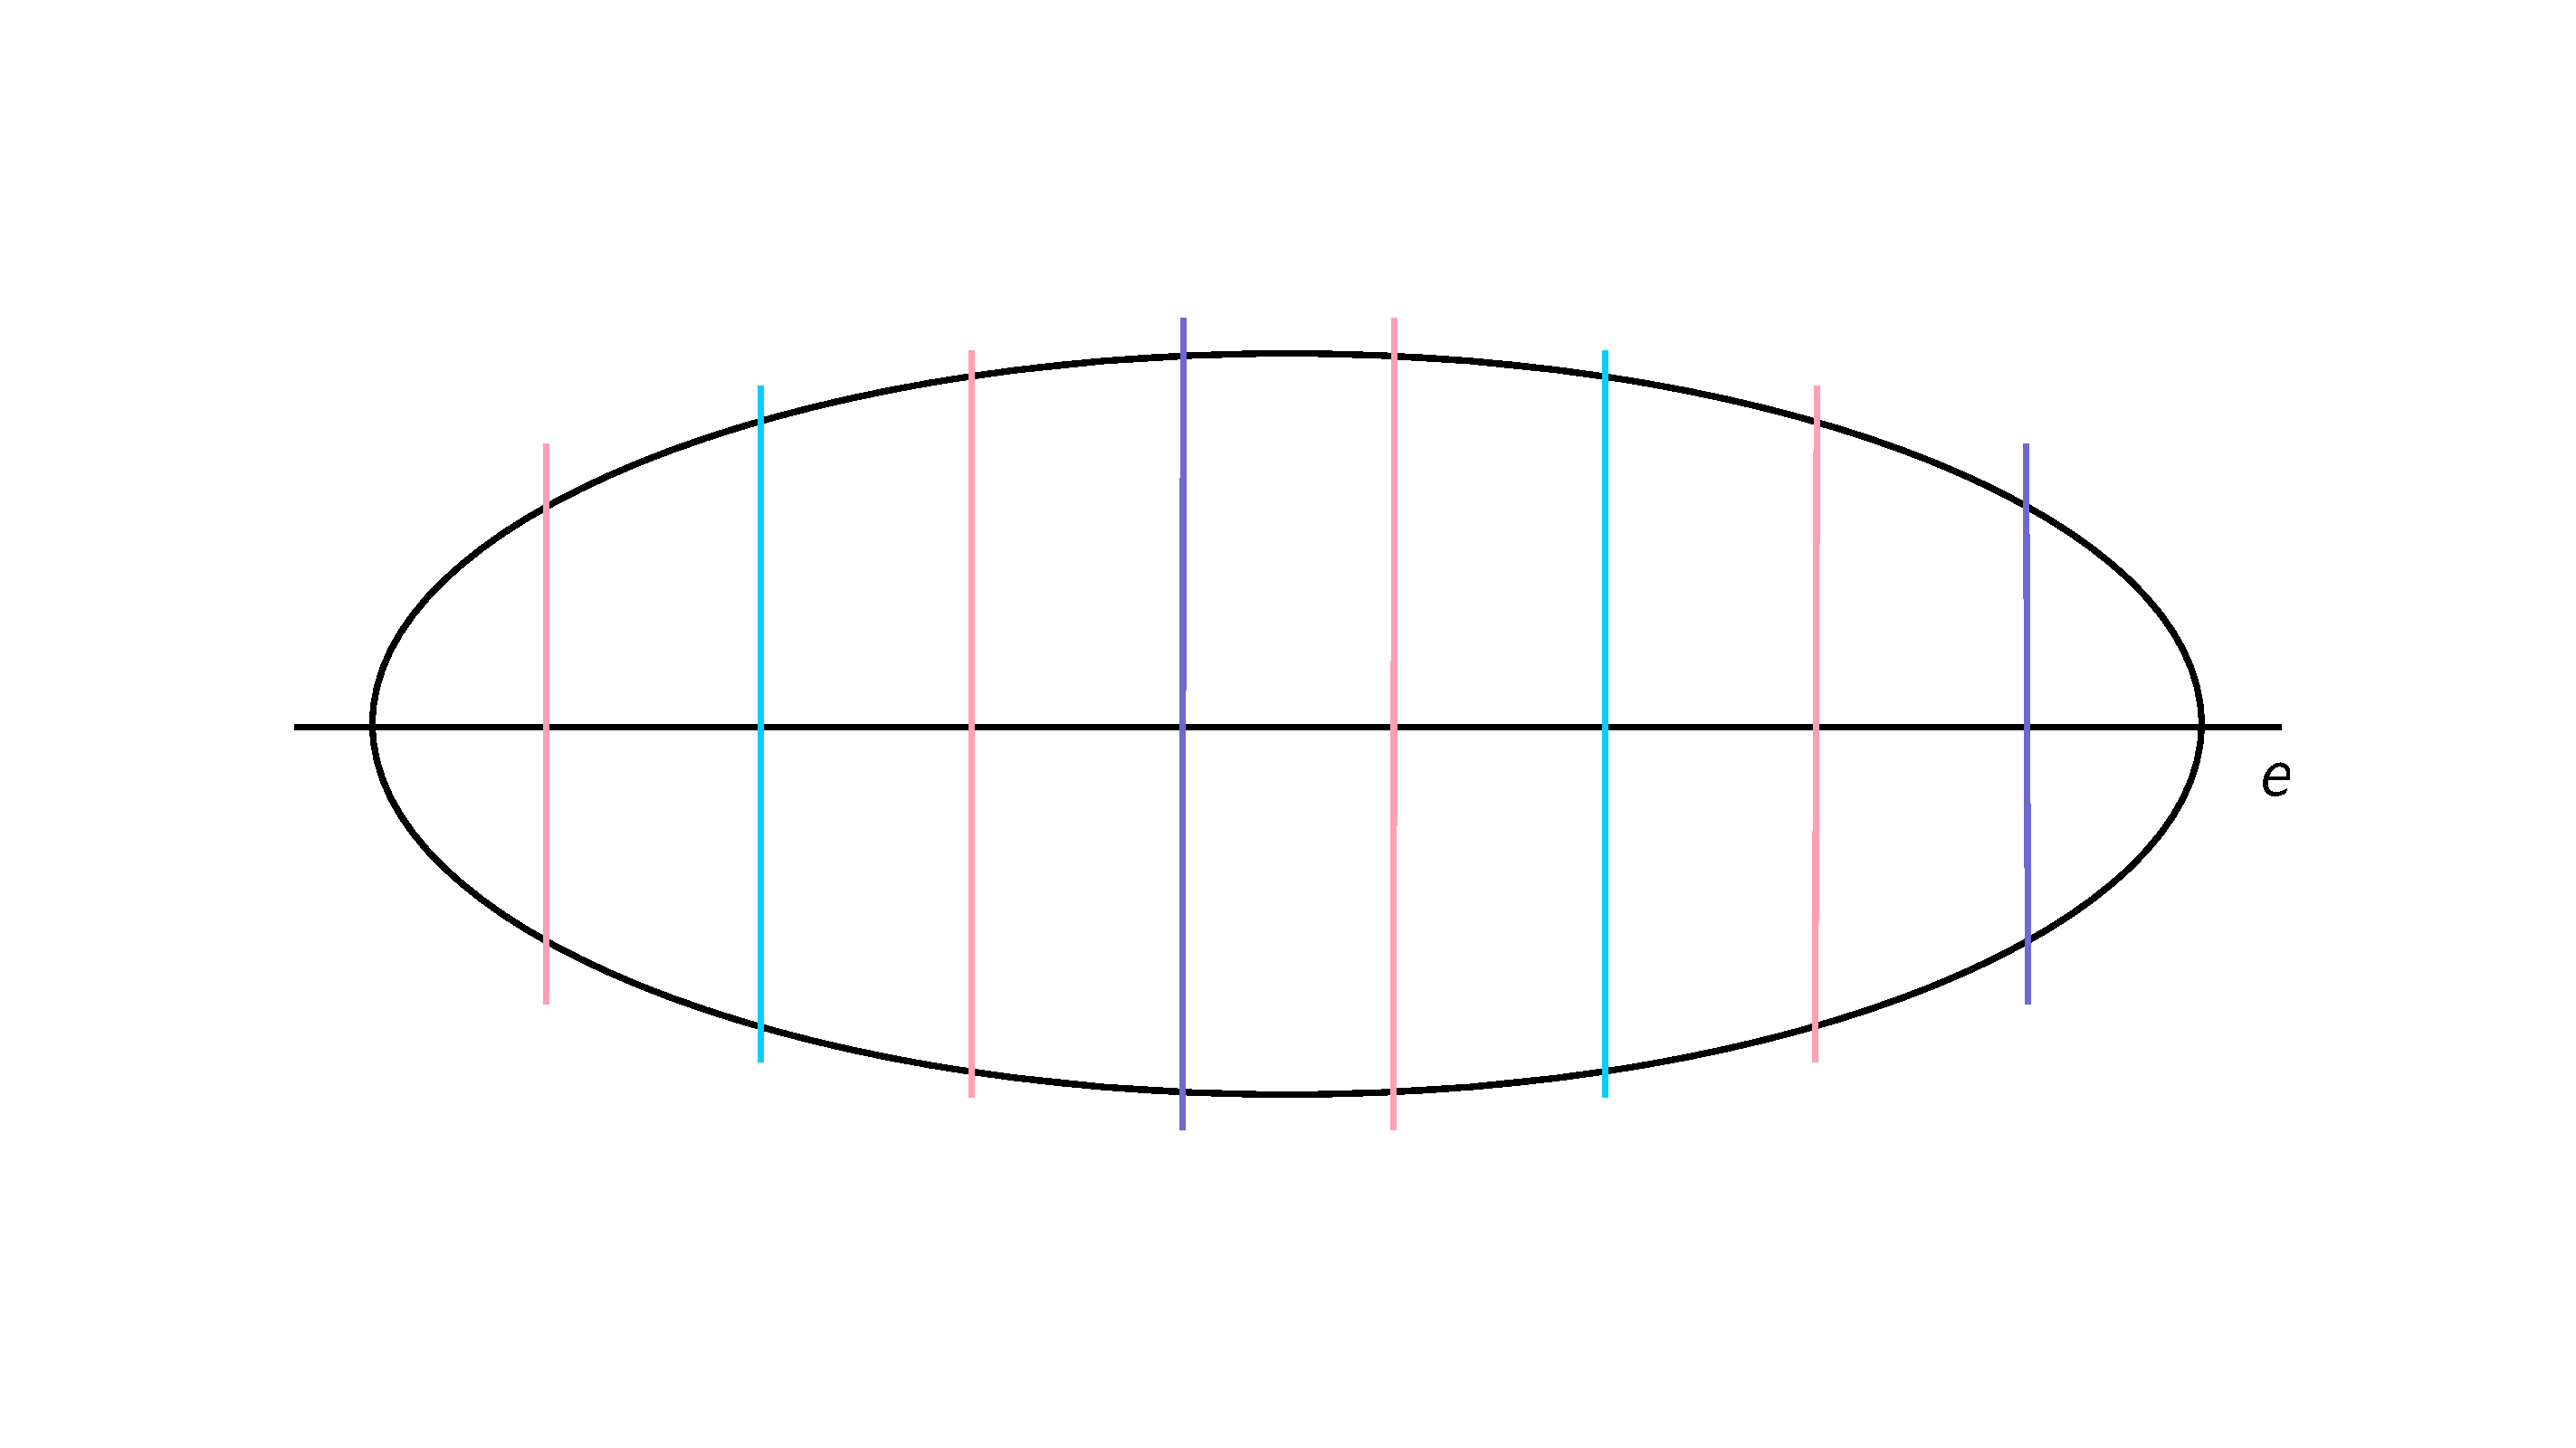
\includegraphics[width=\textwidth]{images/figure-4.pdf}
        \end{center}
    \end{column}
    \end{columns}
\end{frame}

\begin{frame}{Theorem \ref{thm:weak-realizability-bound} Proof}
    \begin{columns}
    \begin{column}{0.35\textwidth}
        \begin{itemize}
            \item Let \(2n_f\) be the number of intersections of edge \(f\) with \(e\) in this window.
            \item<2-> For each \(f\), assign numbers \(1, \ldots, 4 n_f\) to the intersections with the window in the order they appear on \(f\).
            \item<3-> We can assume (by Jordan-Schoenflies theorem) that the window is a circle and \(e\) is a straight line and \(\forall f\), the intersections \(2i-1\) and \(2i\) are mirror images.
        \end{itemize}
    \end{column}
    \begin{column}{0.65\textwidth}
        \begin{center}
            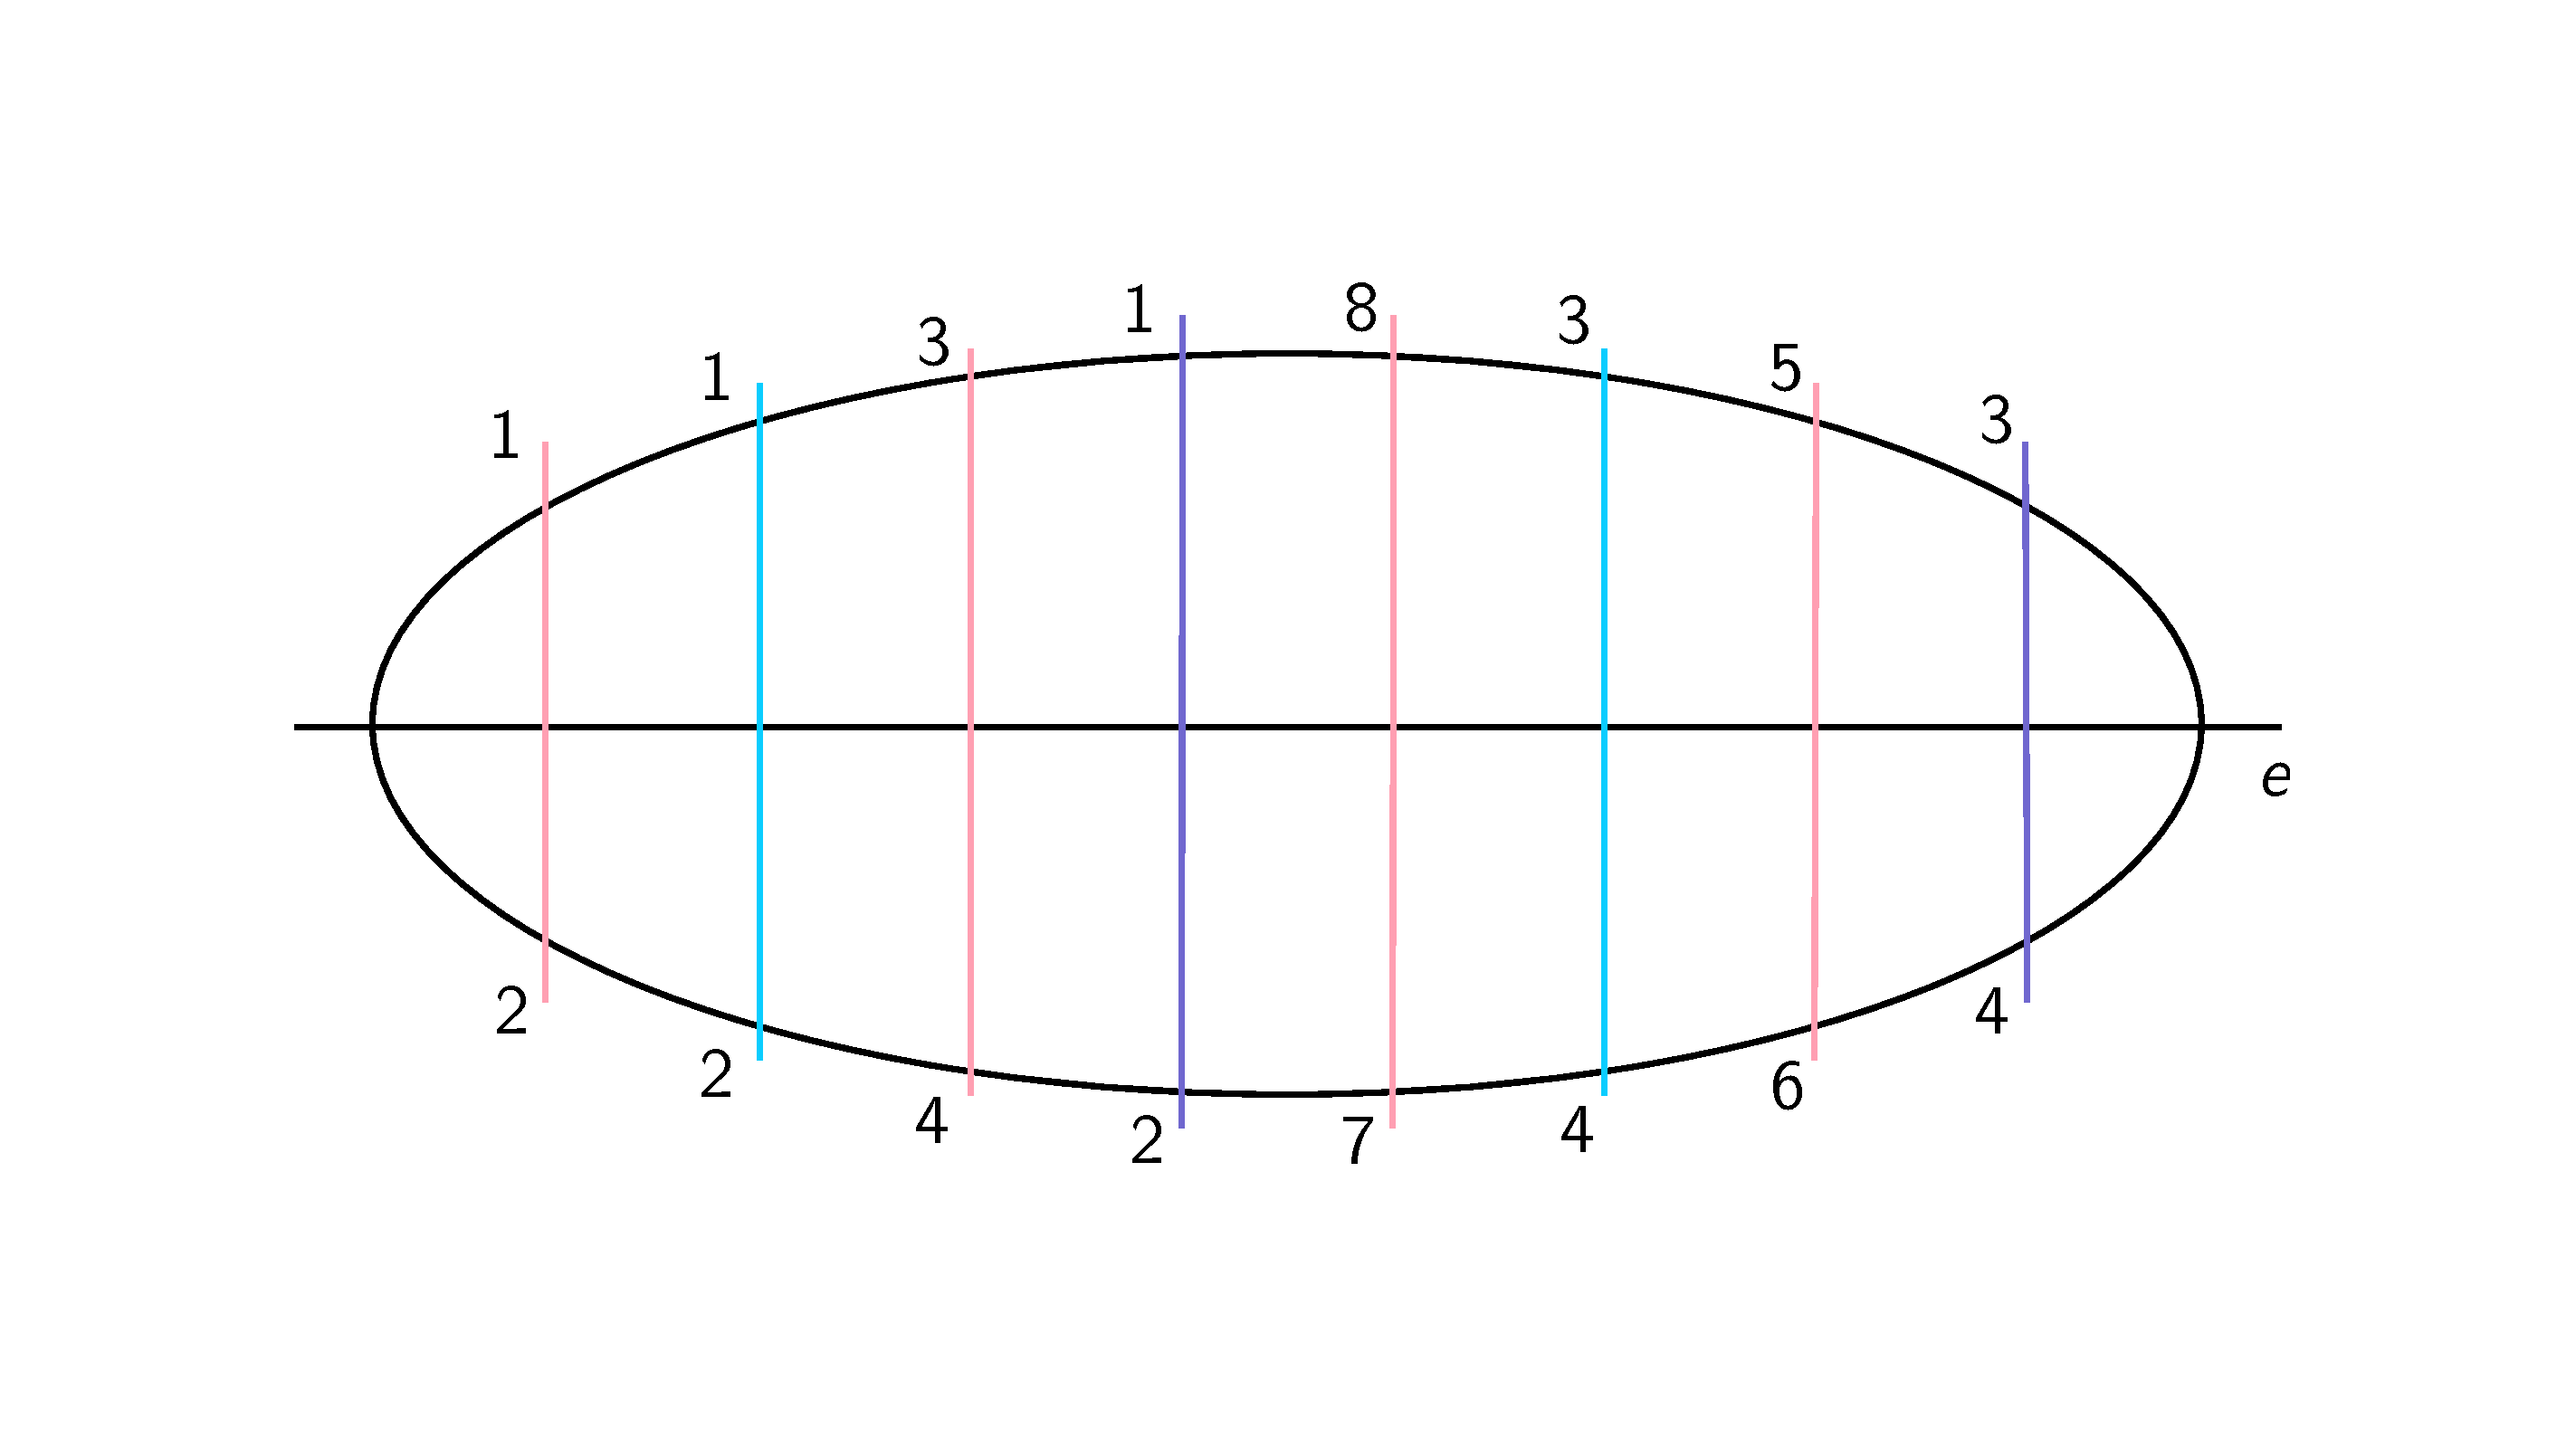
\includegraphics[width=\textwidth]{images/figure-5.pdf}
        \end{center}
    \end{column}
    \end{columns}
\end{frame}

\begin{frame}{Theorem \ref{thm:weak-realizability-bound} Proof}
    \begin{columns}
    \begin{column}{0.35\textwidth}
        \begin{itemize}
            \item For each \(f\), there is a connection between \(4i-2\) and \(4i-1\) (\(i \in \set{1,\ldots, n_f}\)) lying completely outside the window.
        \end{itemize}
    \end{column}
    \begin{column}{0.65\textwidth}
        \begin{center}
            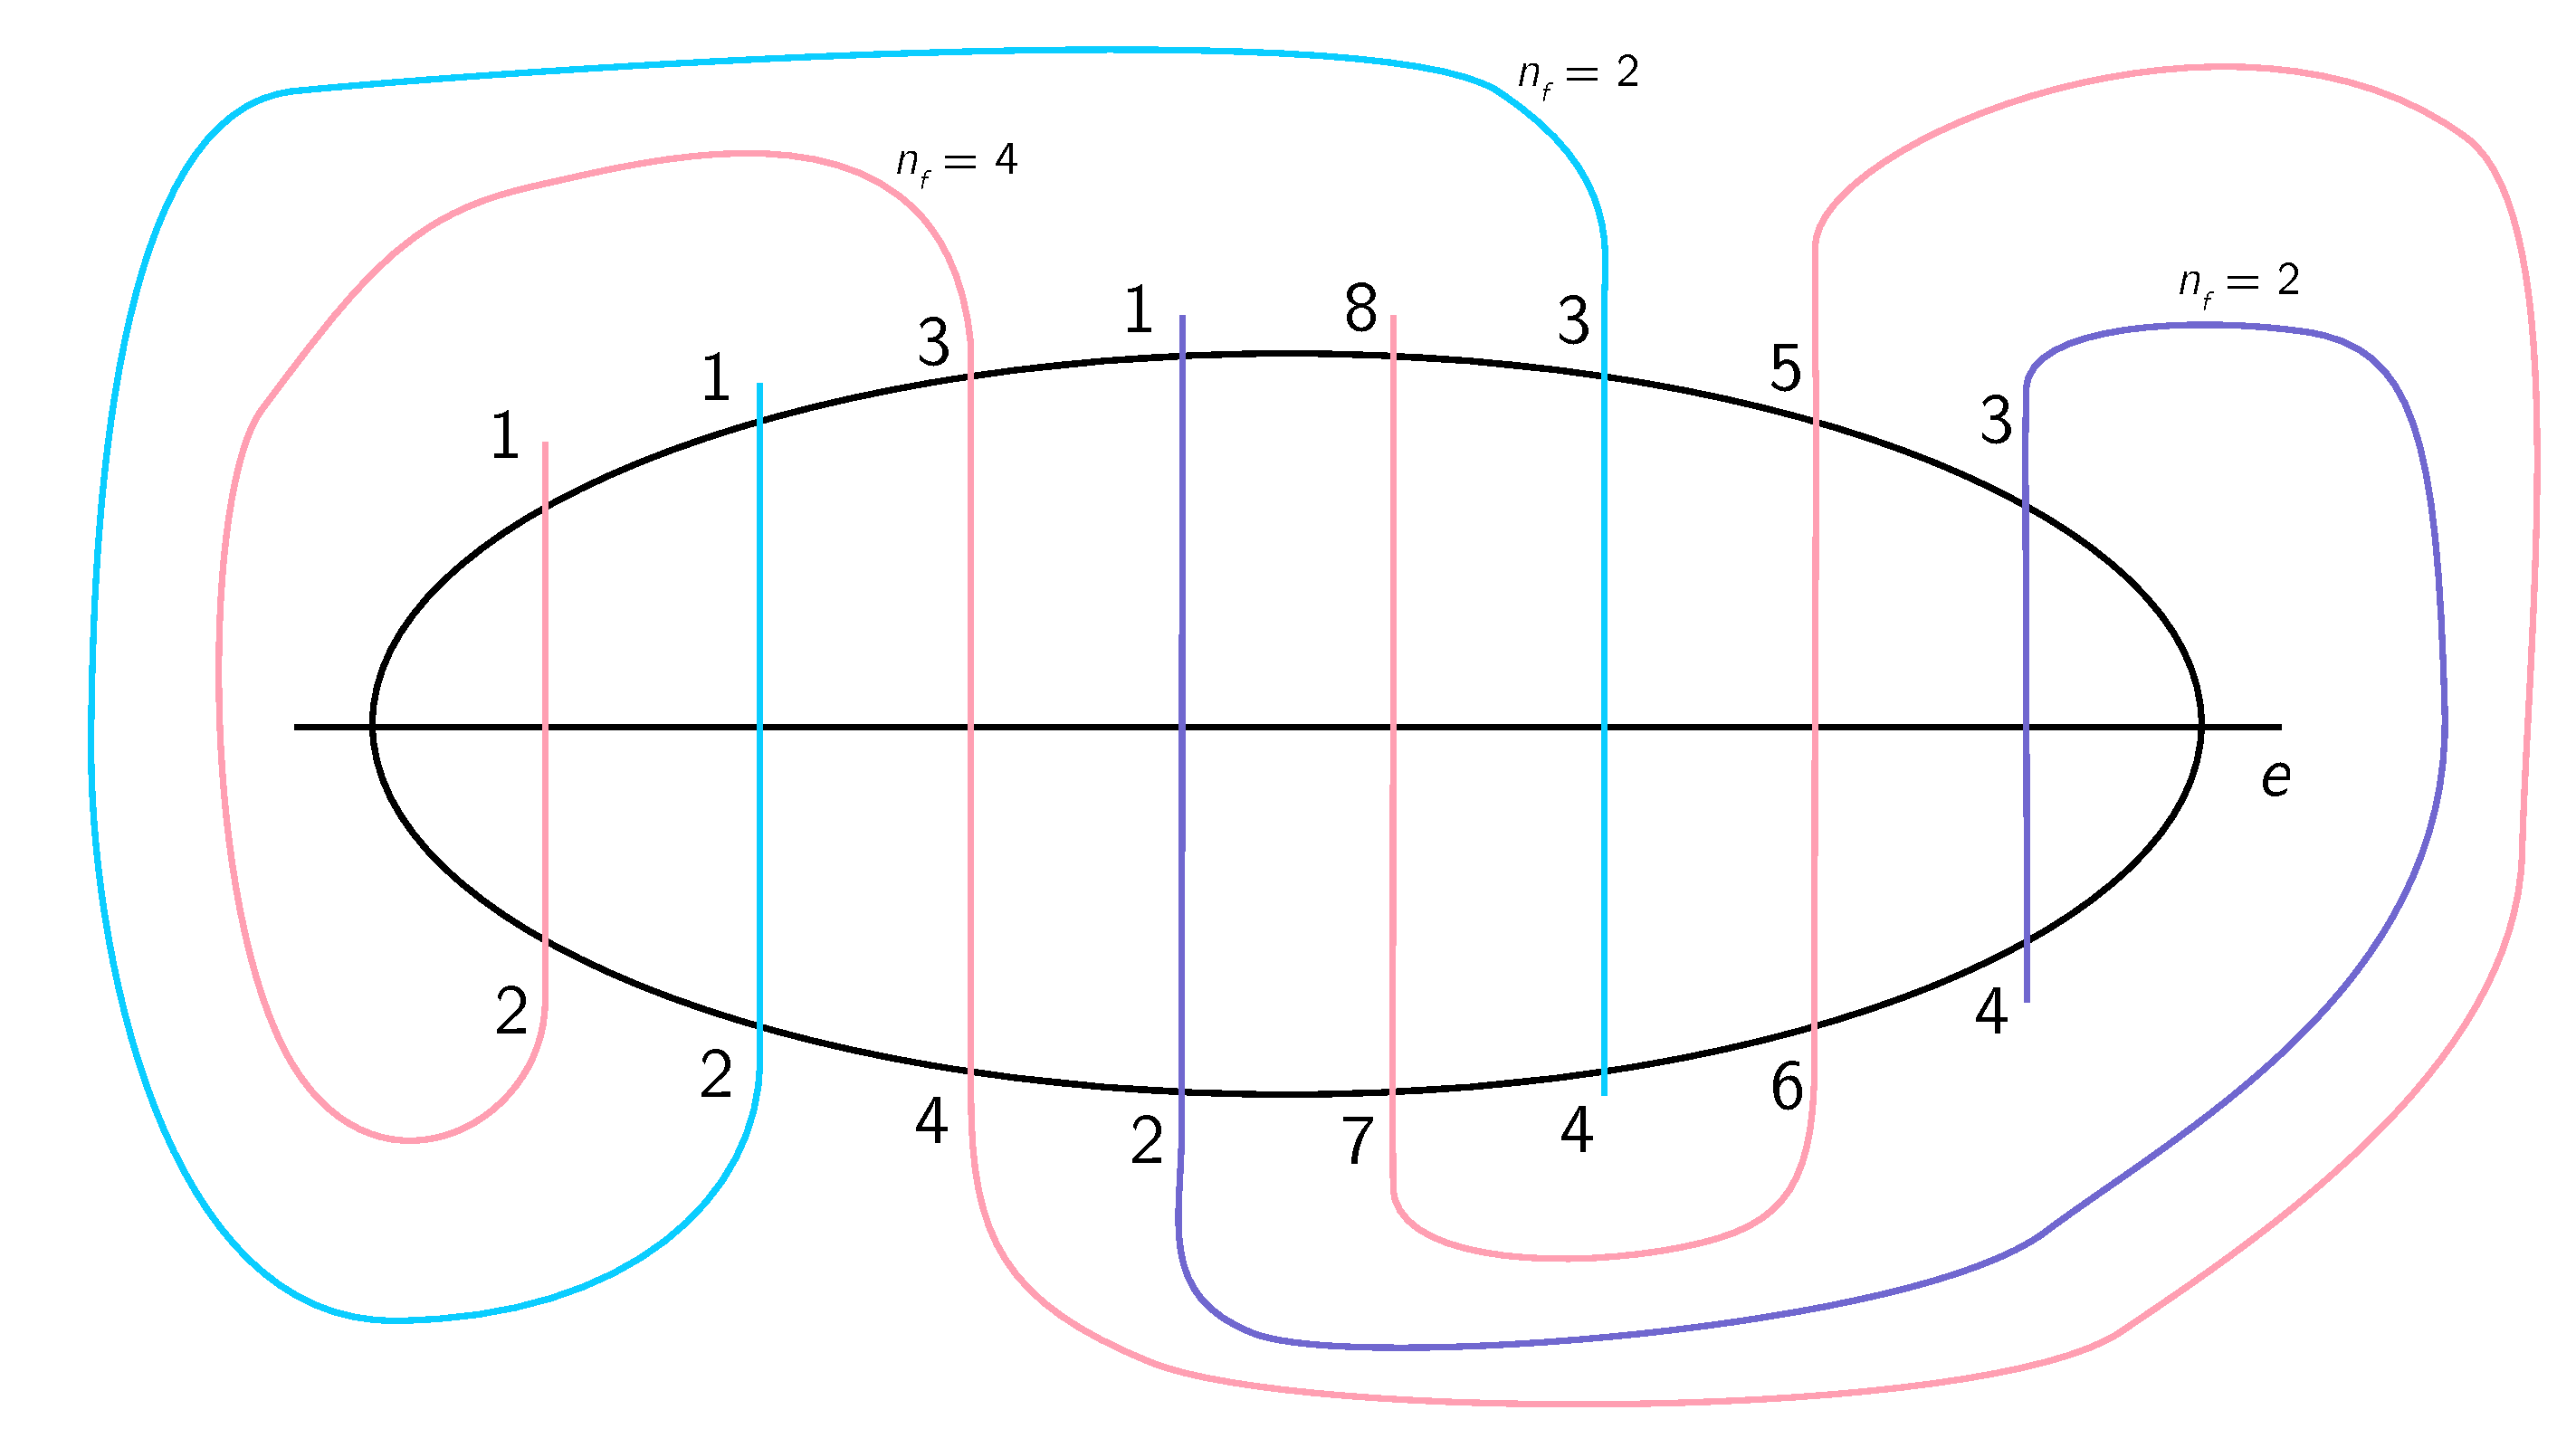
\includegraphics[width=\textwidth]{images/figure-6.pdf}
        \end{center}
    \end{column}
    \end{columns}
\end{frame}

\begin{frame}{Theorem \ref{thm:weak-realizability-bound} Proof}
    \begin{columns}
    \begin{column}{0.35\textwidth}
        \begin{itemize}
            \item Use circular inversion along the circle to bring all of these conections inside.
        \end{itemize}
    \end{column}
    \begin{column}{0.65\textwidth}
        \begin{center}
            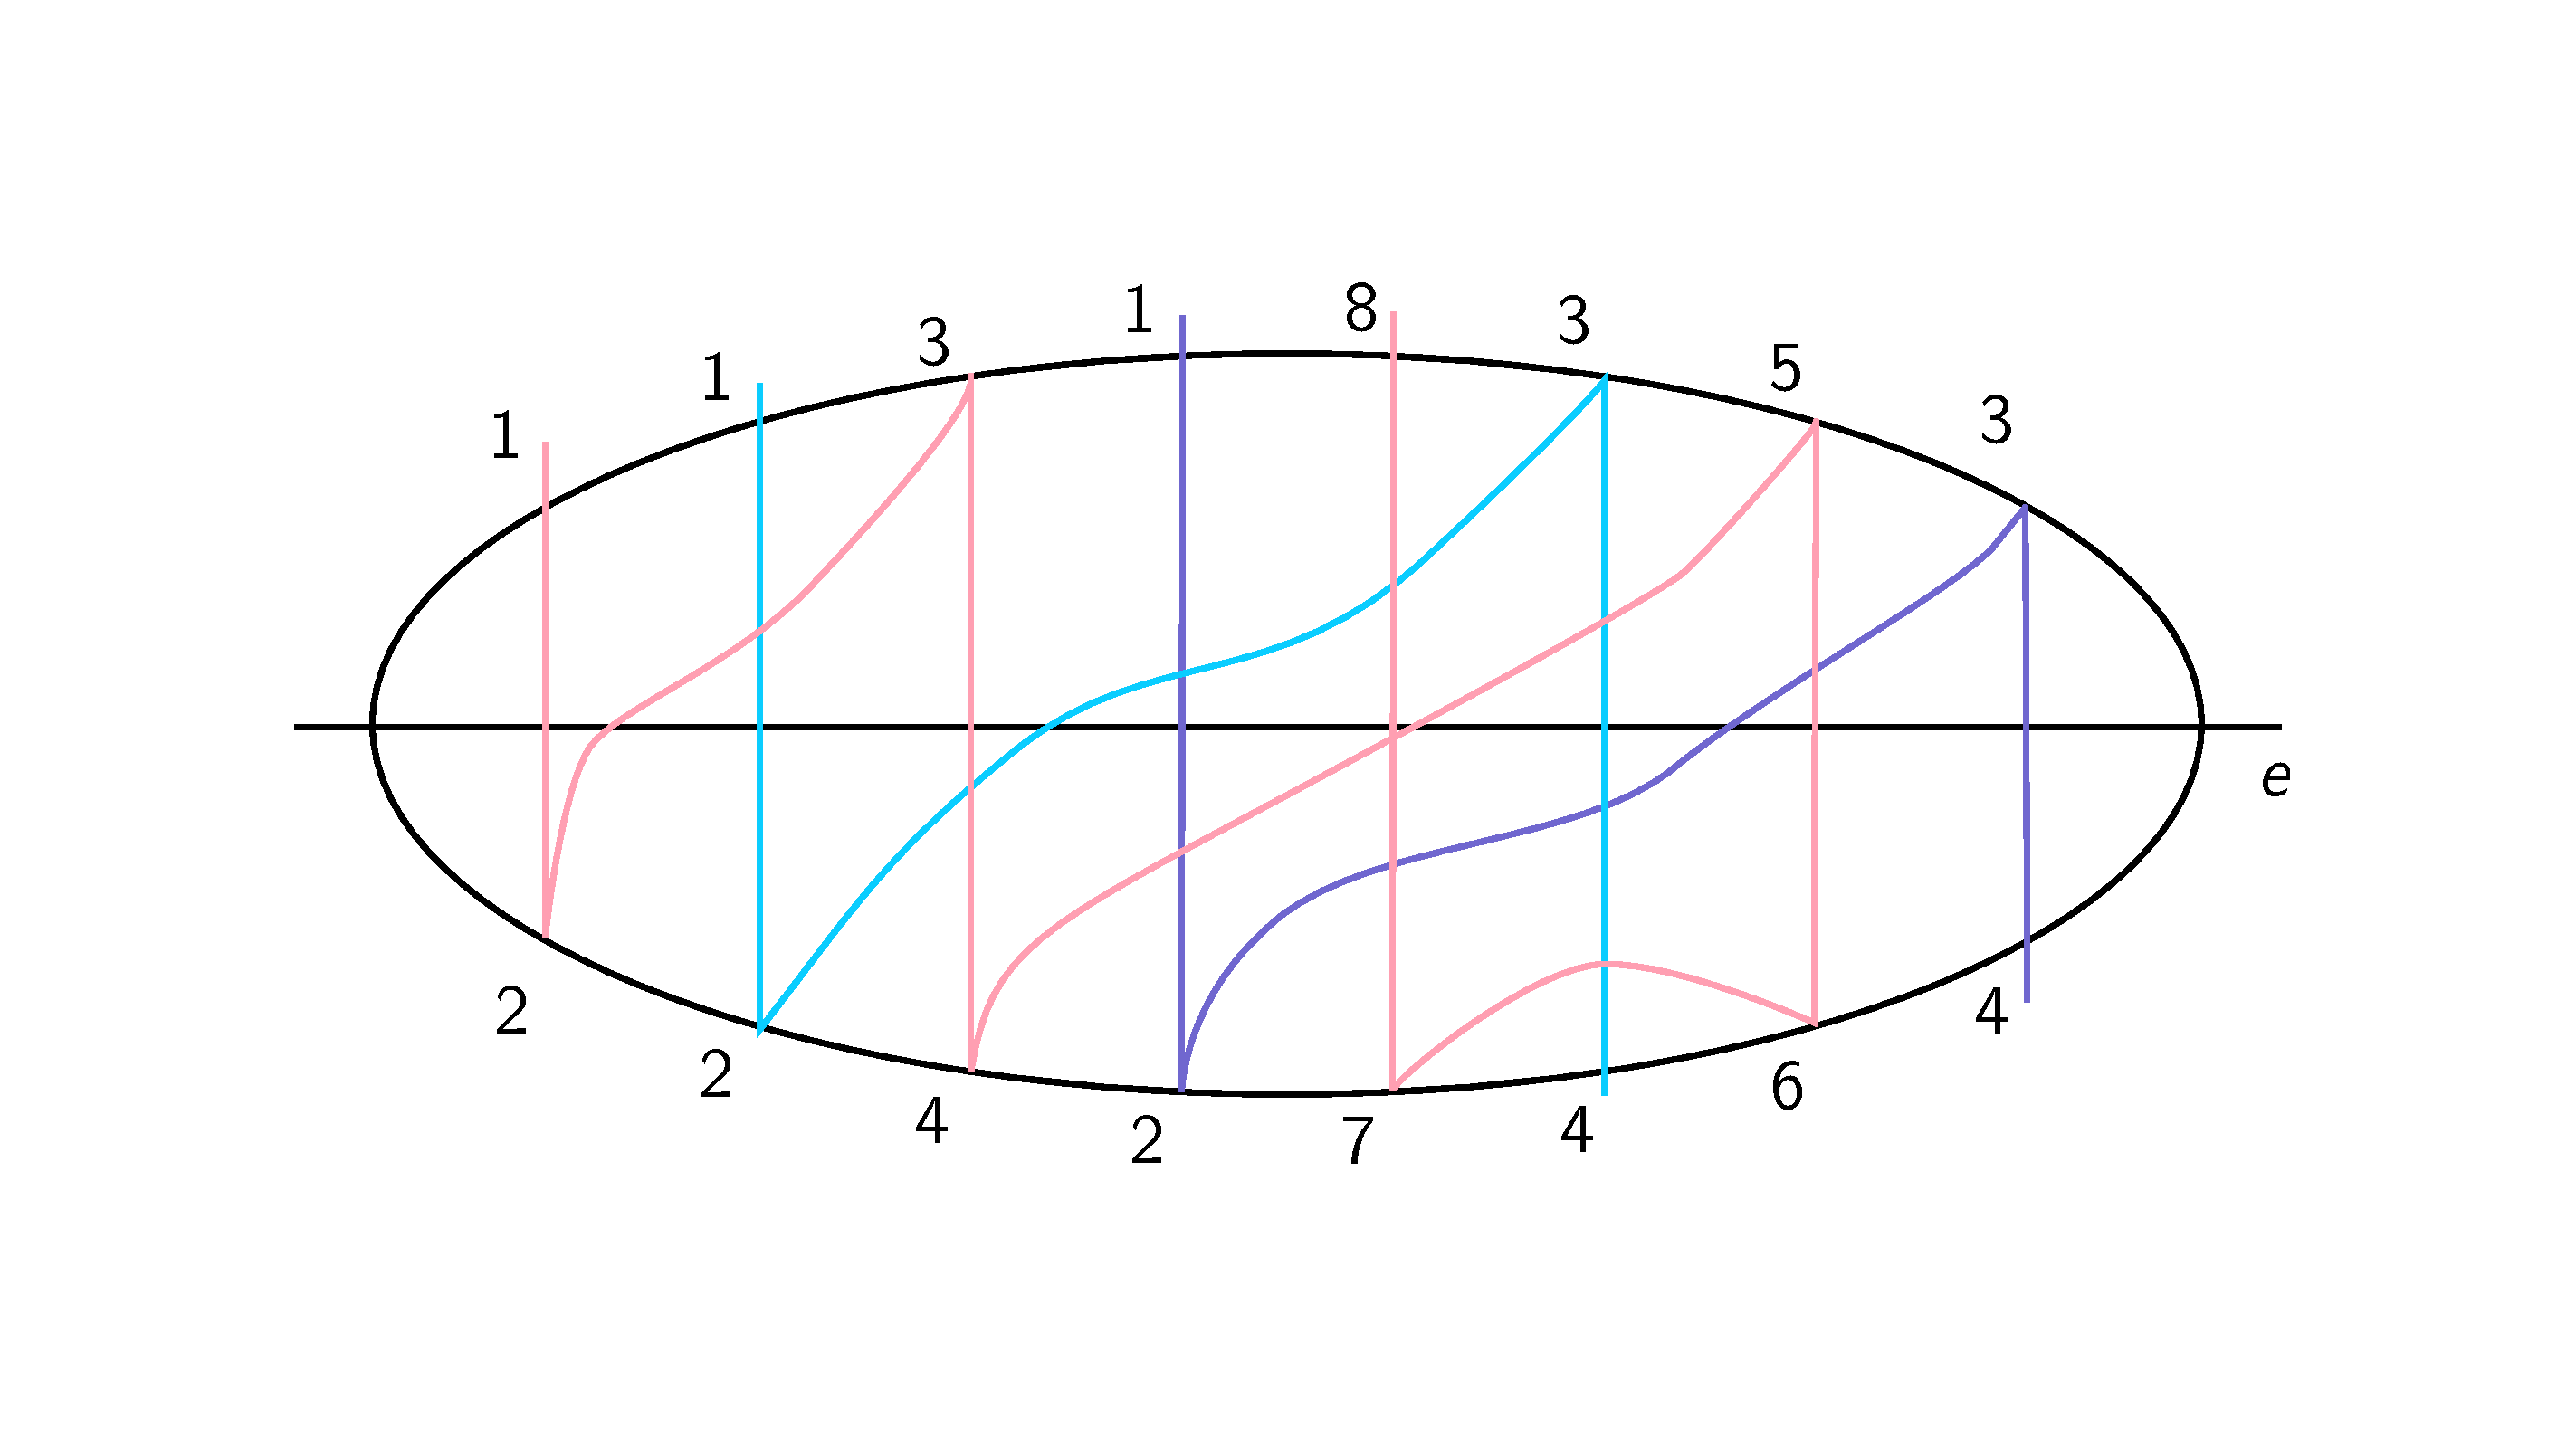
\includegraphics[width=\textwidth]{images/figure-7.pdf}
        \end{center}
    \end{column}
    \end{columns}
\end{frame}

\begin{frame}{Theorem \ref{thm:weak-realizability-bound} Proof}
    \begin{columns}
    \begin{column}{0.35\textwidth}
        \begin{itemize}
            \item Mirror everything inside of the window along \(e\).
        \end{itemize}
    \end{column}
    \begin{column}{0.65\textwidth}
        \begin{center}
            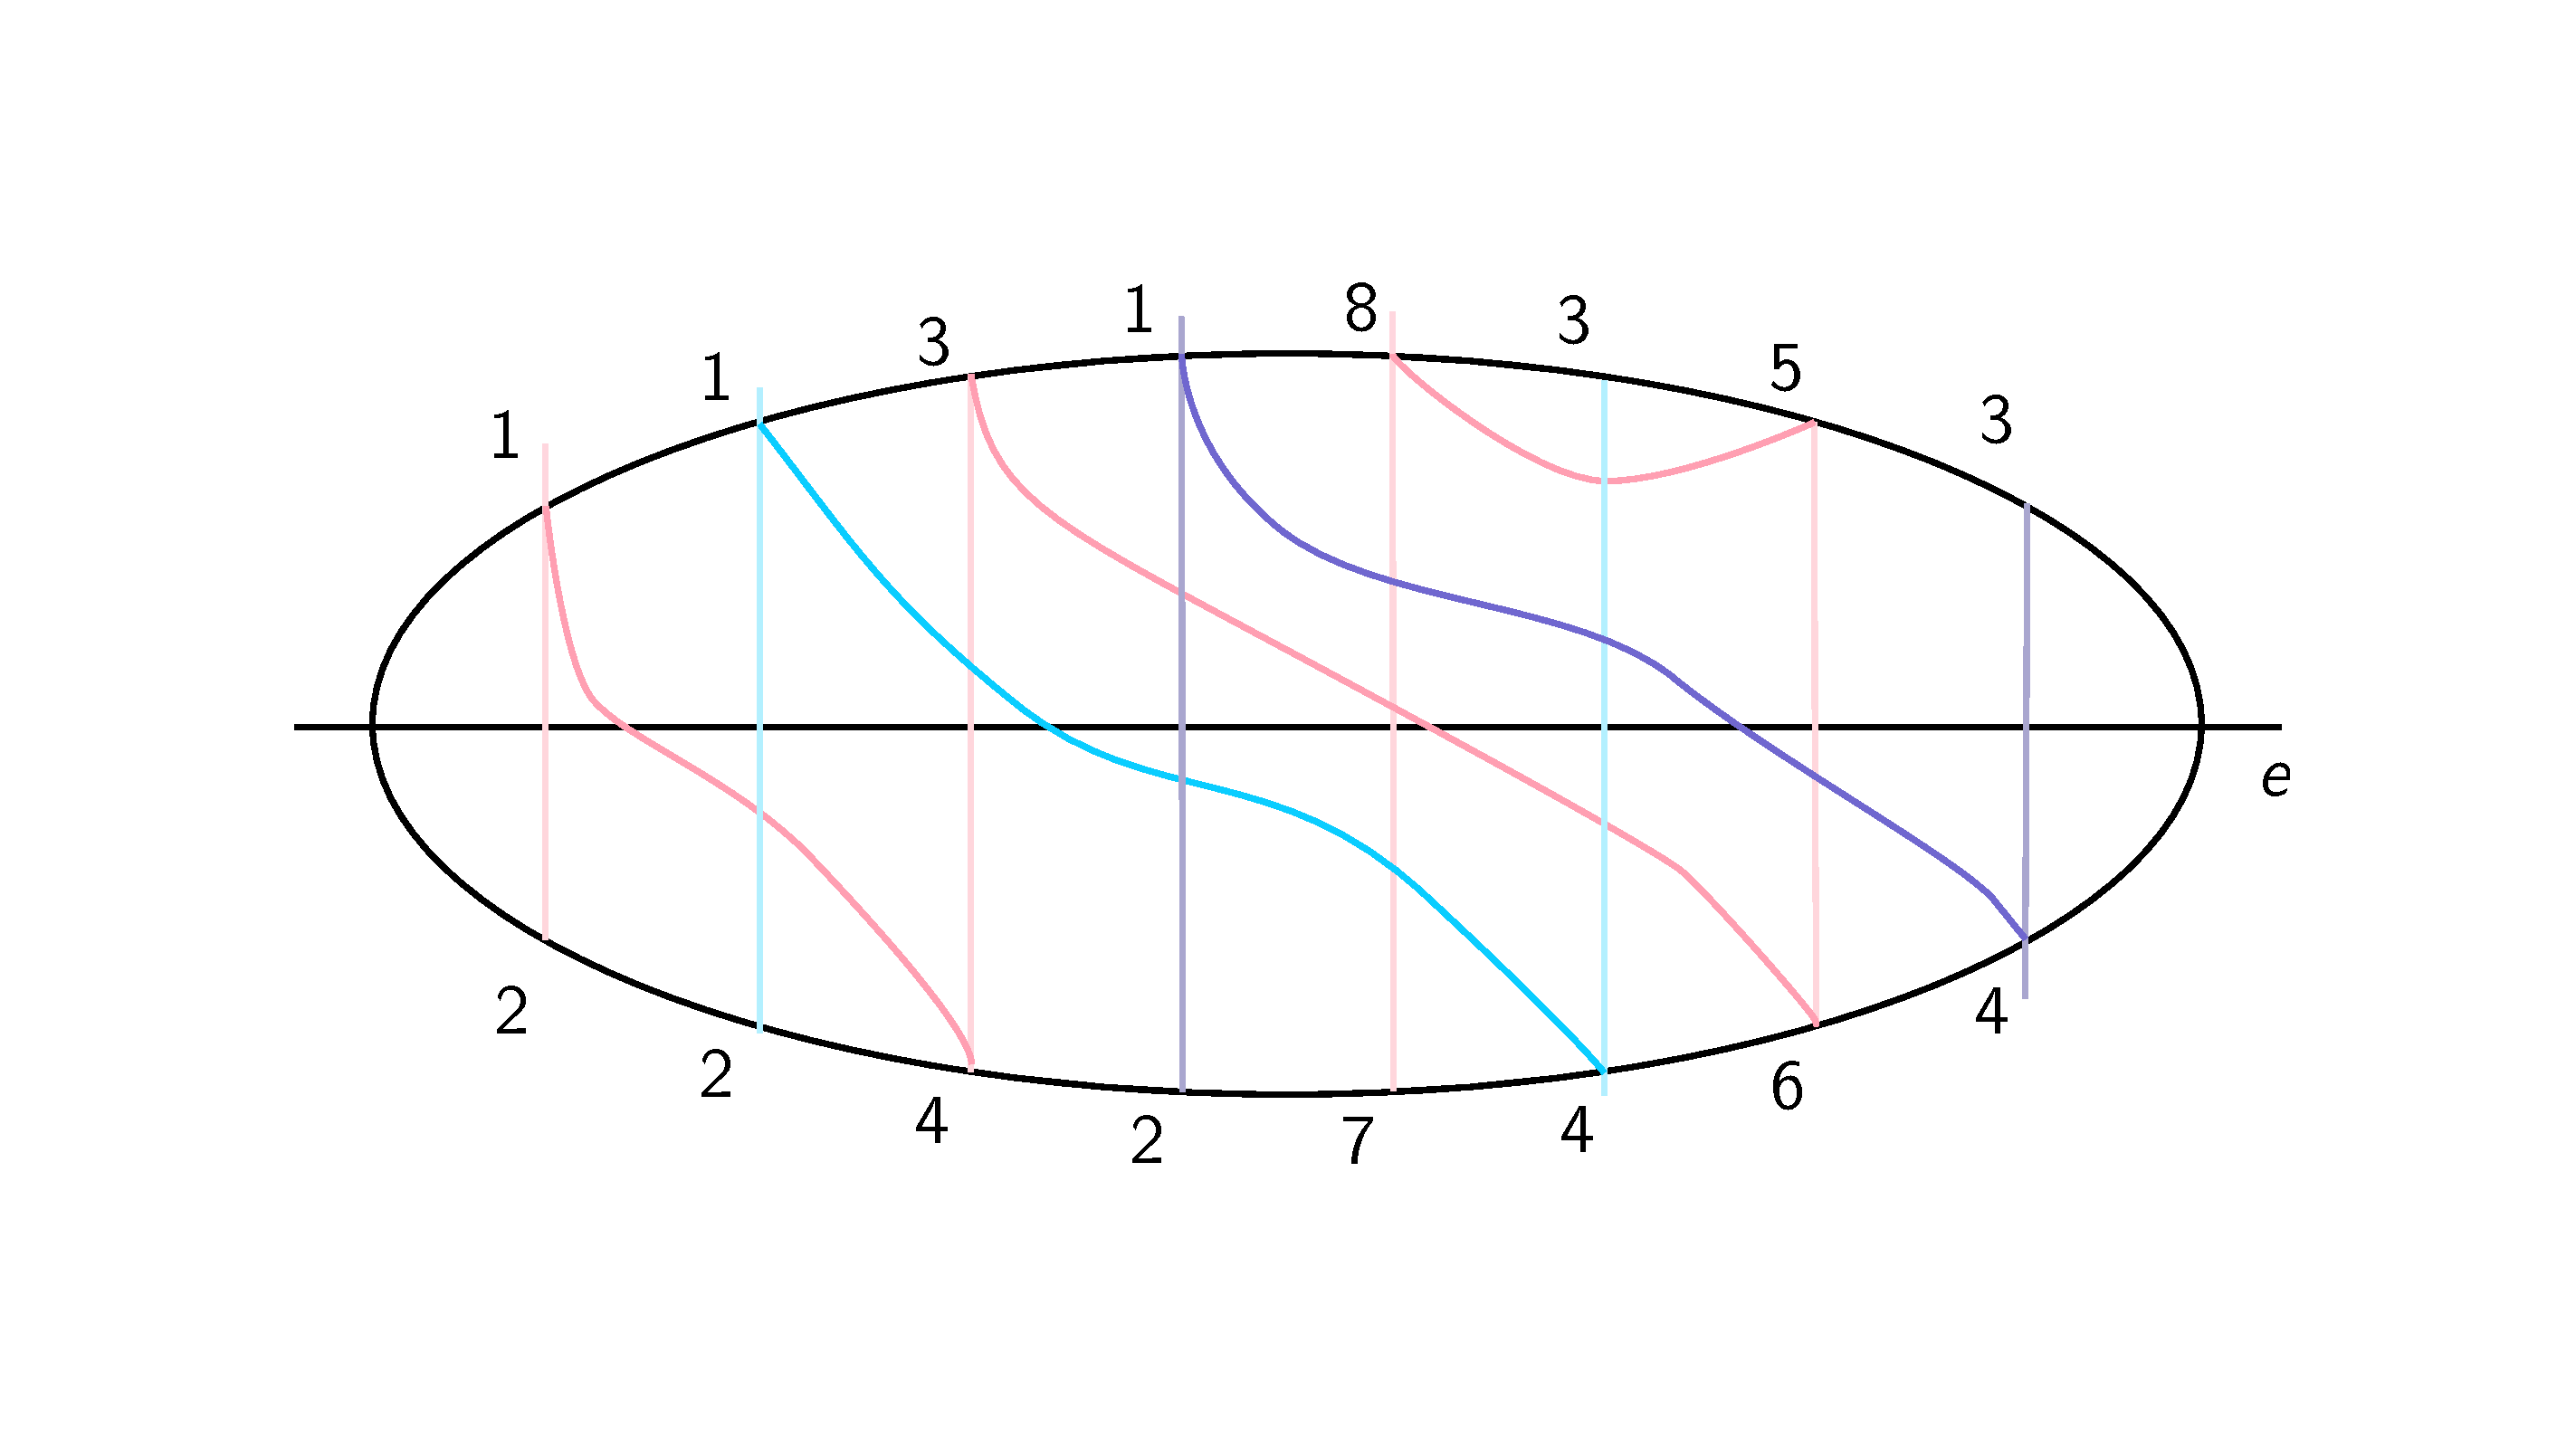
\includegraphics[width=\textwidth]{images/figure-8.pdf}
        \end{center}
    \end{column}
    \end{columns}
\end{frame}

\begin{frame}{Theorem \ref{thm:weak-realizability-bound} Proof}
    \begin{columns}
    \begin{column}{0.35\textwidth}
        \begin{itemize}
            \item Now, we have for every edge a connection between \(4i-3\) and \(4i\) which is inside the window.
            \item<2-> Build a new version \(f'\): start at intersection \(1\) (connected to one of the endpoints of \(f\)), continue to \(4\) (inside), \(5\) (outside), etc. until \(4 n_f\).            
        \end{itemize}
    \end{column}
    \begin{column}{0.65\textwidth}
        \begin{center}
            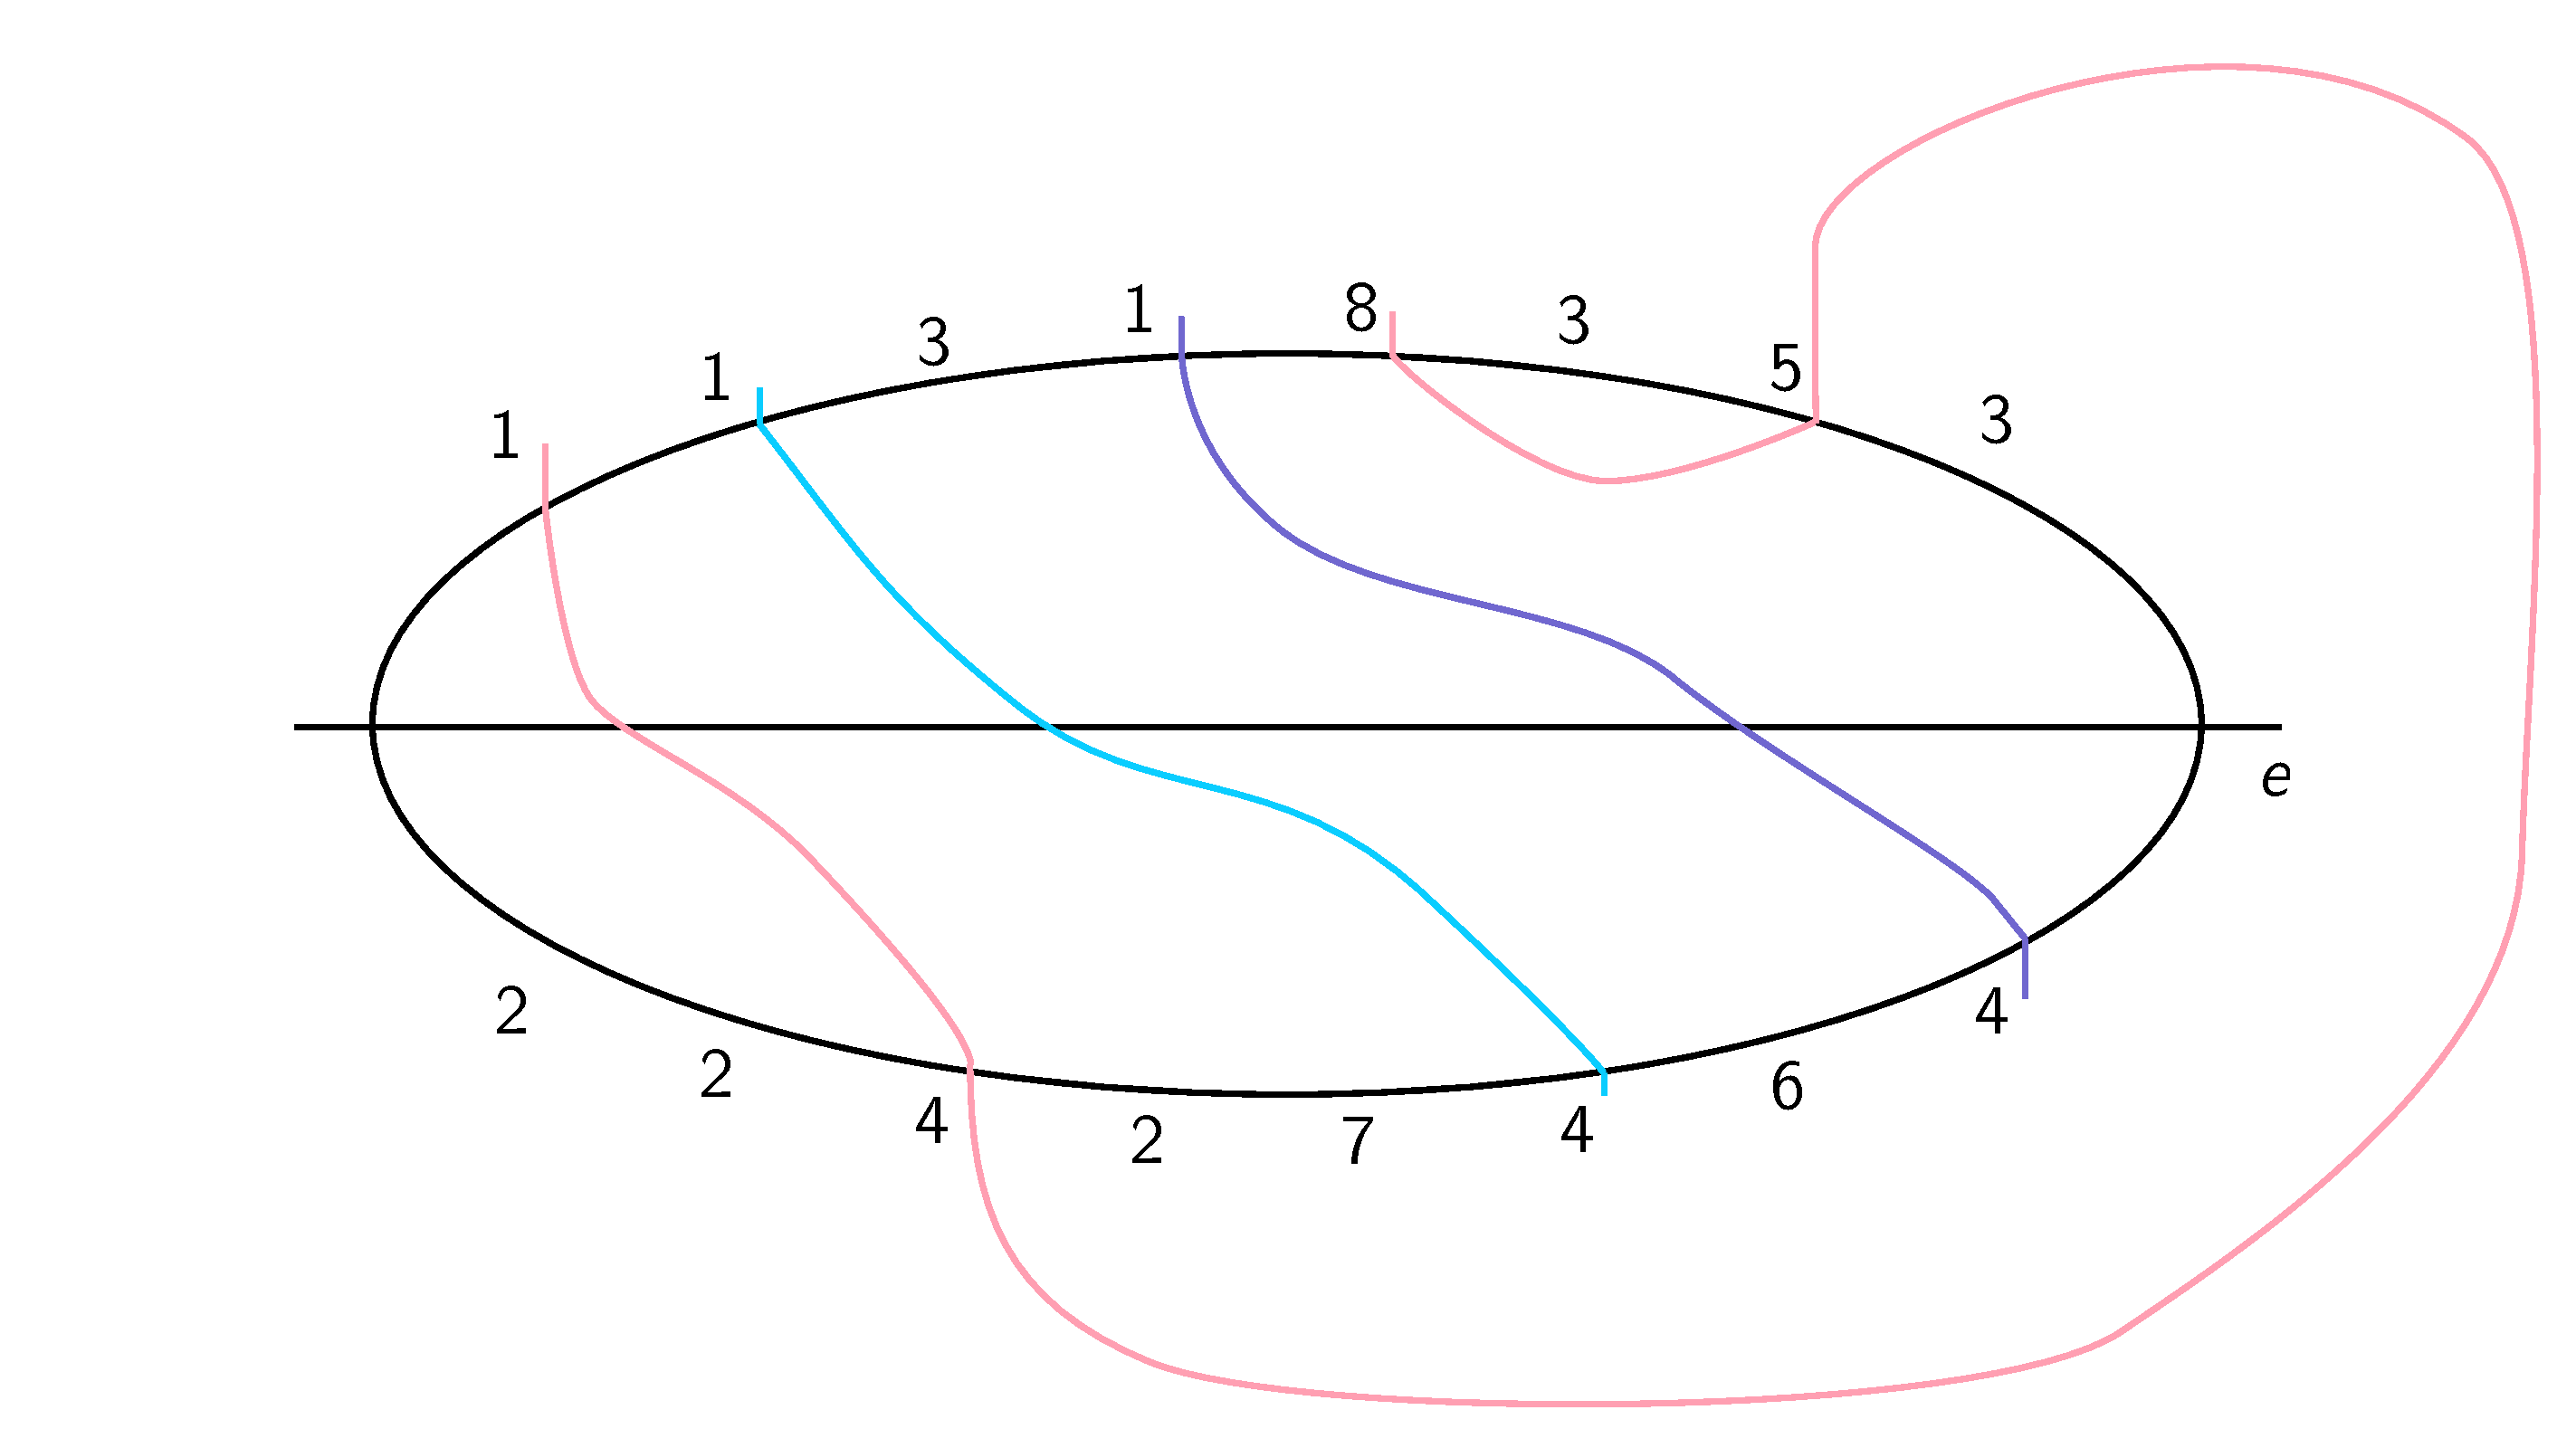
\includegraphics[width=\textwidth]{images/figure-9.pdf}
        \end{center}
    \end{column}
    \end{columns}
\end{frame}

\begin{frame}{Theorem \ref{thm:weak-realizability-bound} Proof}
    \begin{columns}
    \begin{column}{0.35\textwidth}
        \begin{itemize}
            \item \(f\) intersects \(e\) an even number of times \(\Rightarrow f'\) still connects the two original endpoints.
            \item<2-> \(\leadsto\) reduced the number of intersections with the window from \(4 n_f\) to \(2 n_f\).
            \item<3-> Every intersection between the curves inside the circle corresponds to an intersection outside \(\Rightarrow\) the new realization respects \(R\) (in this example, there are no intersections).
        \end{itemize}
    \end{column}
    \begin{column}{0.65\textwidth}
        \begin{center}
            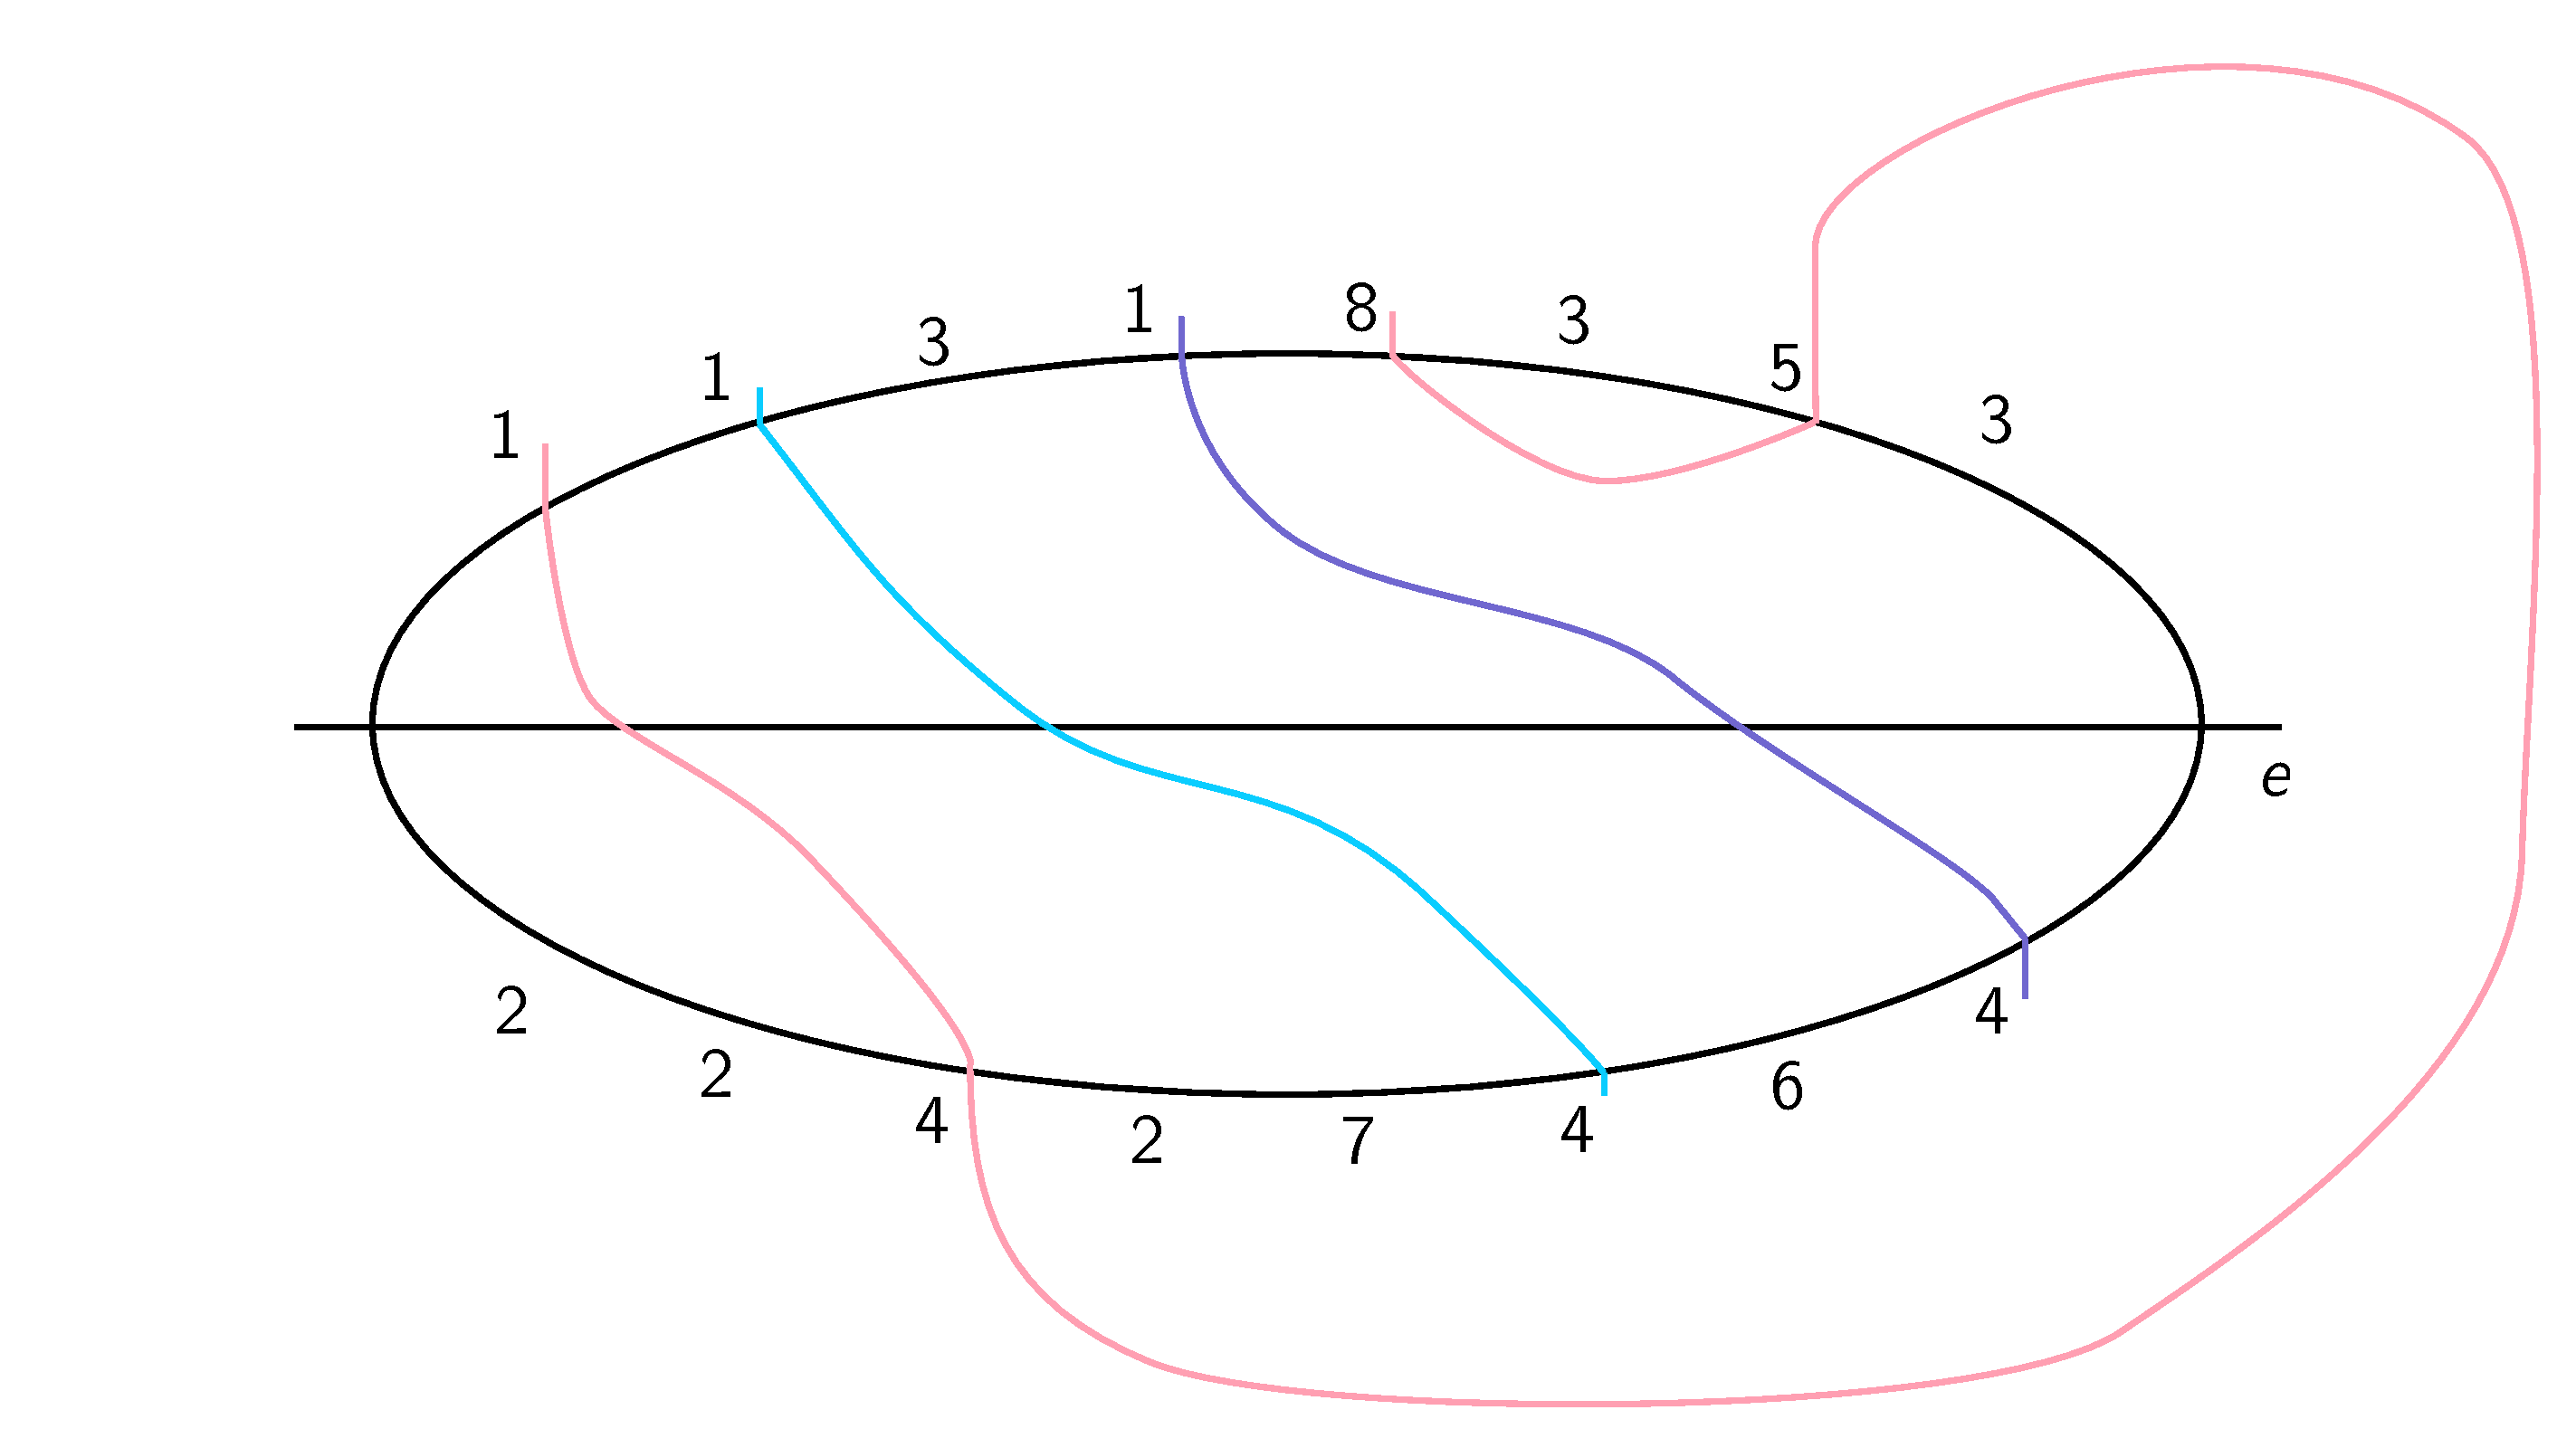
\includegraphics[width=\textwidth]{images/figure-9.pdf}
        \end{center}
    \end{column}
    \end{columns}
\end{frame}

\begin{frame}{Theorem \ref{thm:weak-realizability-bound} Proof}
    \begin{columns}
    \begin{column}{0.35\textwidth}
        \begin{itemize}
            \item The number of intersections along \(e\) might have increased.
            \item<2-> \(f'\) halved the number of intersections between the \(f'\) and the window boundary. 
            \item<3-> \(\leadsto\) \(e' \coloneqq\) one of the two sides of the boundary of the window (at least one side has less intersections than before). \qed
        \end{itemize}
    \end{column}
    \begin{column}{0.65\textwidth}
        \begin{center}
            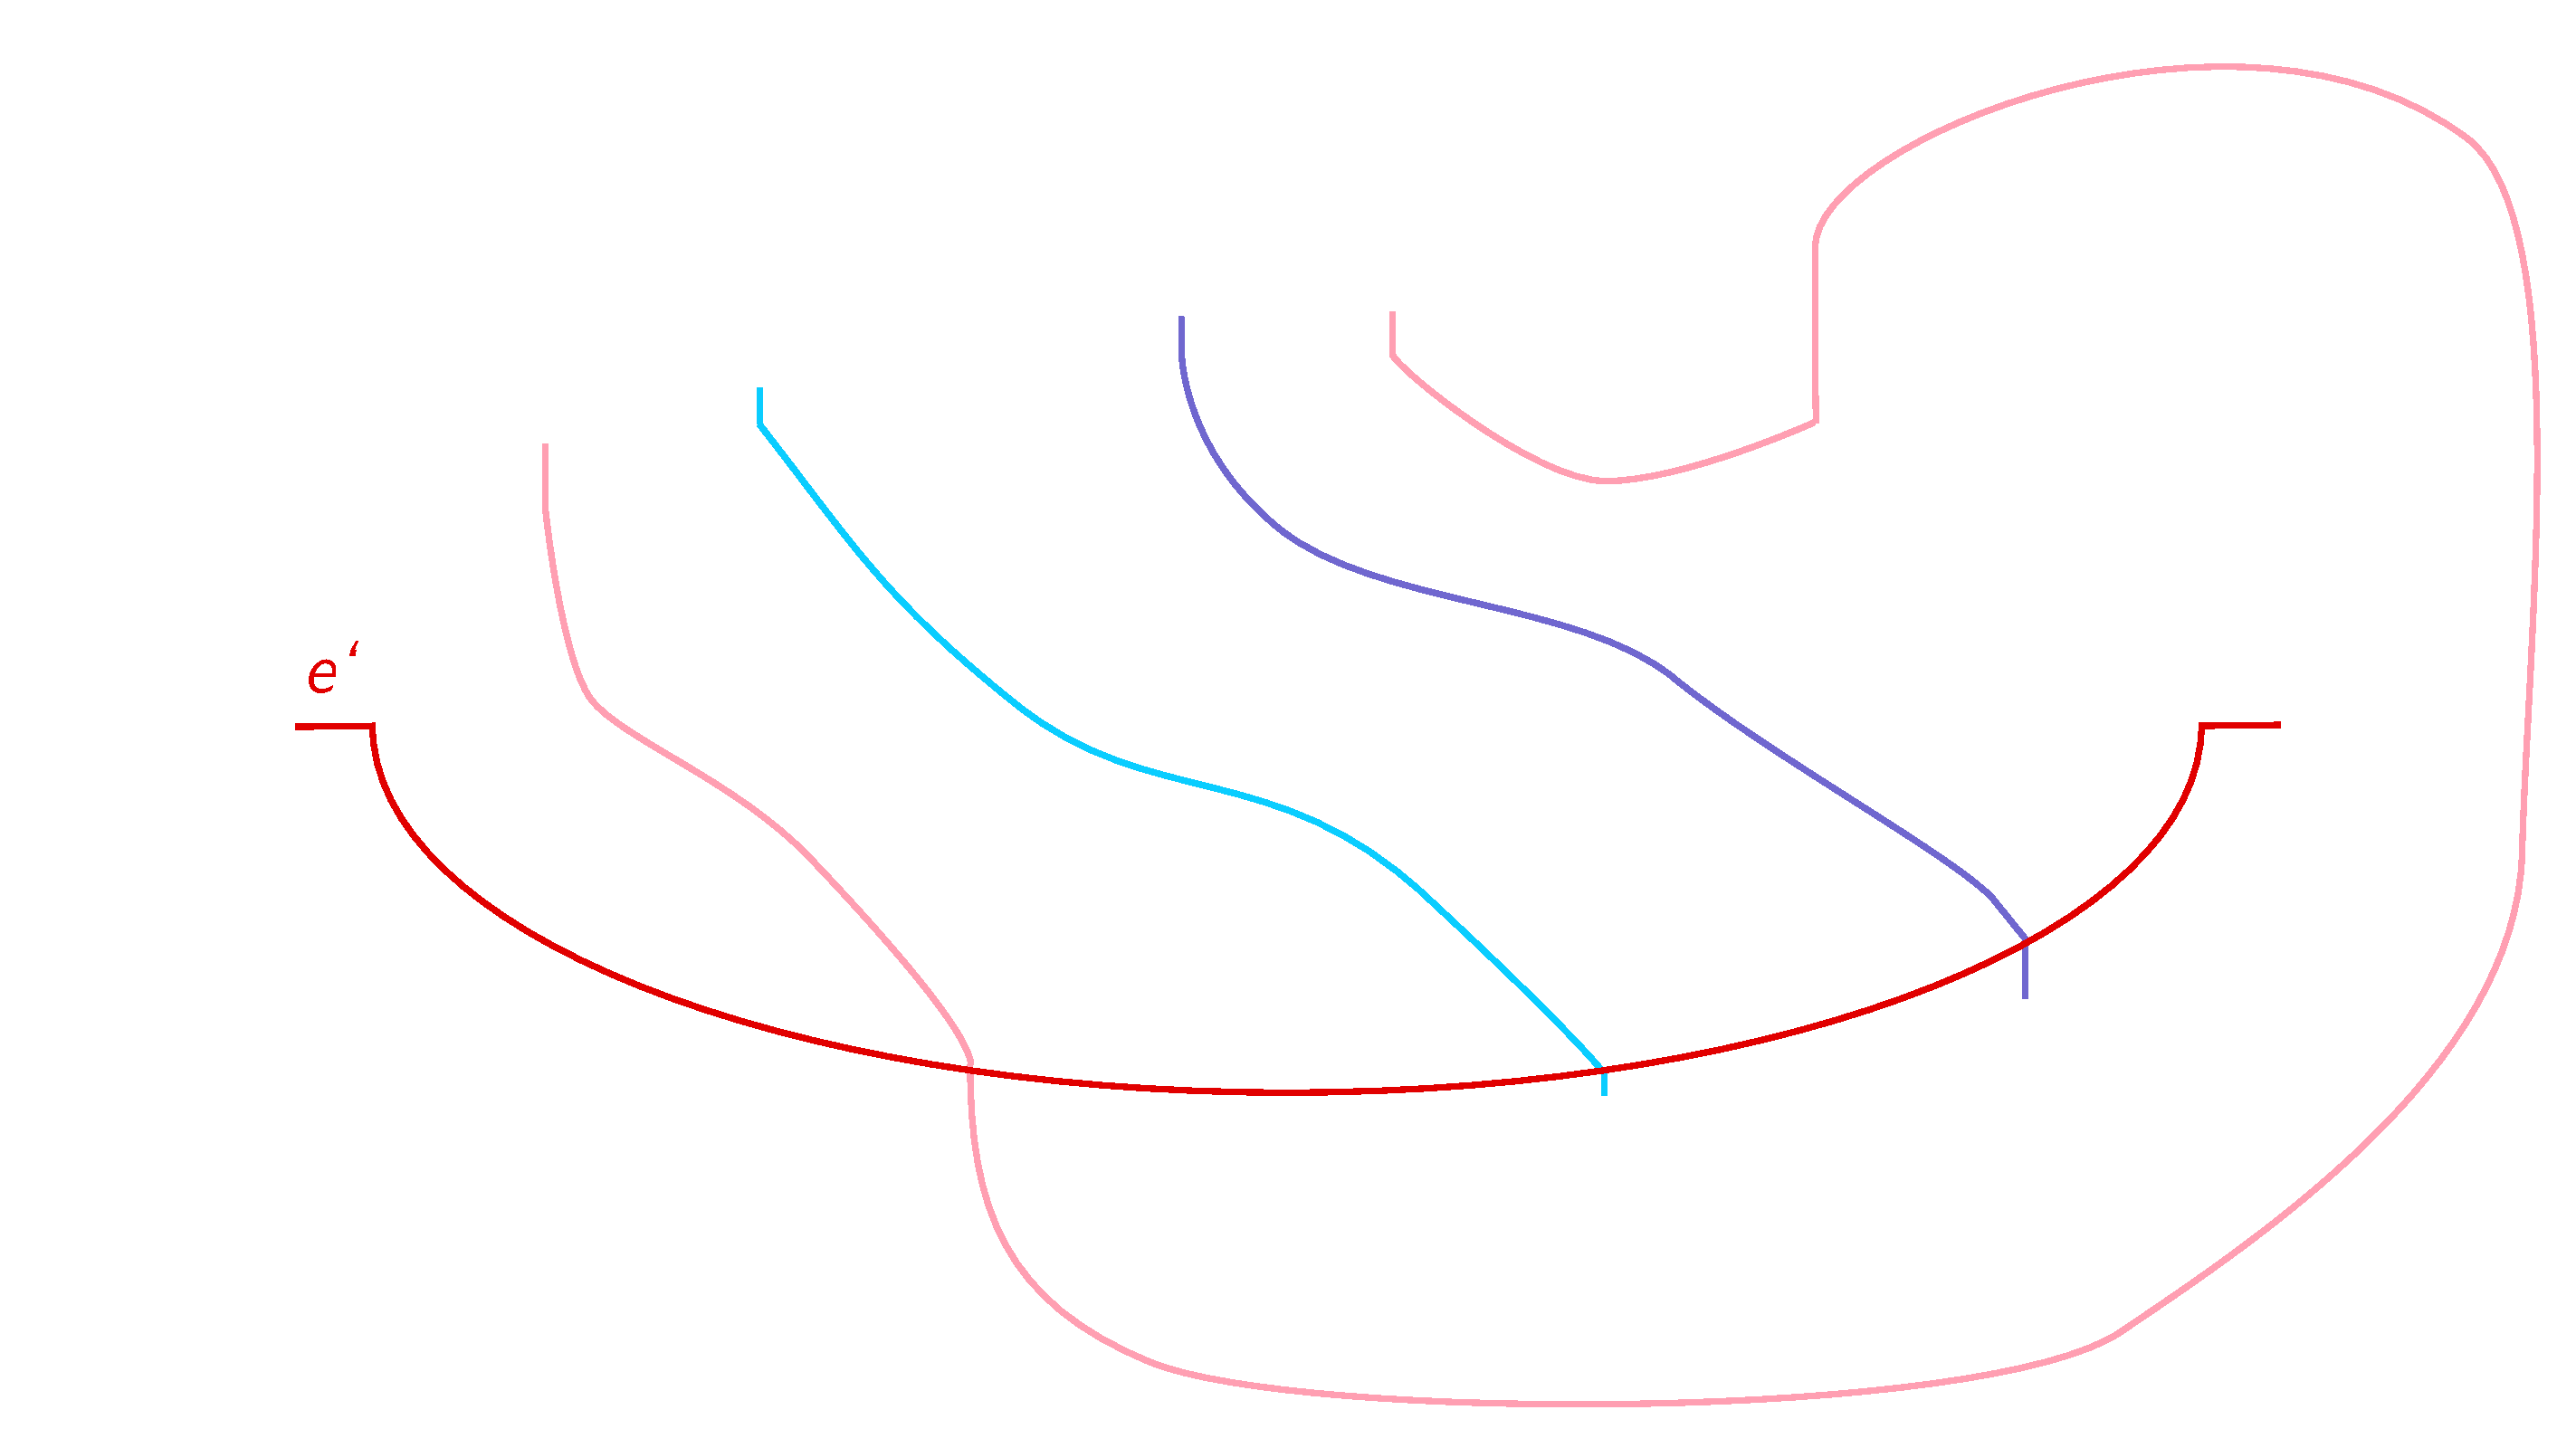
\includegraphics[width=\textwidth]{images/figure-10.pdf}
        \end{center}
    \end{column}
    \end{columns}
\end{frame}

\begin{frame}{String graph decidability}
    \begin{corollary}
        String graph recognition is in \(\mathbf{NEXP}\).
        \label{cor:decidability}
    \end{corollary}
    \begin{theorem}[Schnyder]
        Each plane graph with \(n \geq 3\) vertices has a straight line embedding on the \(n-2\) by \(n-2\) grid.
    \end{theorem}
\end{frame}

\addtocounter{theorem}{-2}
\begin{frame}[t]{Corollary \ref{cor:decidability} Proof}
    \begin{corollary}
        String graph recognition is in \(\mathbf{NEXP}\).
    \end{corollary}
    \begin{theorem}[{{\color<5>{highlight}Schnyder}}]
        Each plane graph with \(n \geq 3\) vertices has a straight line embedding on the \(n-2\) by \(n-2\) grid.
        \label{thm:schnyder}
    \end{theorem}
    \begin{itemize}
        \item Let \(G\) be a string graph with \(m\) vertices. \pause
        Then, since \(c_s(m) \leq 4 c_w(2m) + 2m\), generate an instance \((G', R)\) with \(c m\) vertices for some \(c > 0\) s.t.
        \((G', R)\) is weakly realizable.
        \item<3-> Using Theorem \ref{thm:weak-realizability-bound}, there must be a drawing with \(\leq 2^{cm}\) intersections per edge.\\
        \(\leadsto\) The collection of curves also has \(M \leq 2^{\tilde{c} m}\) intersections.
        \item<4-> Consider this collection of curves of size \(M\) and draw them as a plane graph \\(intersection \(\mapsto\) vertex), at most \(M\) vertices.
        \item<5-> By Theorem \ref{thm:schnyder}, there is a drawing of this graph on an \((M-2) \times (M-2)\) grid.
        \item<6-> \(\Rightarrow\) in \(\mathbf{NEXP}\), guess a graph (\(\sim\) collection of curves) on such a grid and verify whether its intersection graph is isomorphic to \(G\). \qed
    \end{itemize}
\end{frame}

\section{String Graphs Requiring Exponential Representations \cite{kra91a}}

\begin{frame}{String Graphs Requiring Exponential Representations}
    Goal: provide a construction of a graph on \(O(n)\) vertices which can be represented
    as a string graph but every realization of the graph requires an exponential number of intersections.

    \(\leadsto\) for string graph testing, we need to check at least exponentially many realizations
\end{frame}

\begin{frame}{Exponential Representations}
    \begin{theorem}
        \(c_w(m) \geq 2^{c m}\) for some constant \(c > 0\).
        \label{thm:exp-cw}
    \end{theorem}
\end{frame}

\begin{frame}{Theorem \ref{thm:exp-cw} Proof}
    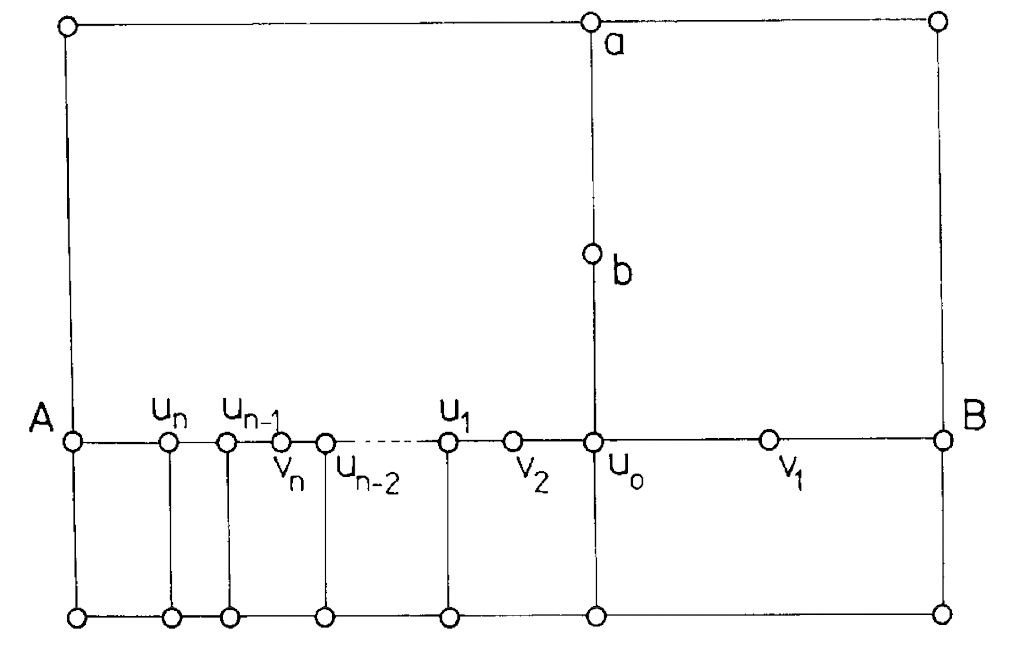
\includegraphics[width=0.8\textwidth]{images/figure-11.png}
\end{frame}

\addtocounter{theorem}{-1}
\begin{frame}[t]{Theorem \ref{thm:exp-cw} Proof}
    \begin{theorem}
        \(c_w(m) \geq 2^{c m}\) for some constant \(c > 0\).
    \end{theorem}
    \begin{columns}
        \begin{column}{0.5\textwidth}
            \begin{itemize}
                \item This graph has a topologically unique drawing.
                \item Add edges \(\set{u_i, v_i}, i=1,2,\ldots, n \), allow them to cross only the edge \(\set{a,b}\) and the horizontal path \(AB\), not each other.
            \end{itemize}
        \end{column}
        \begin{column}{0.5\textwidth}
            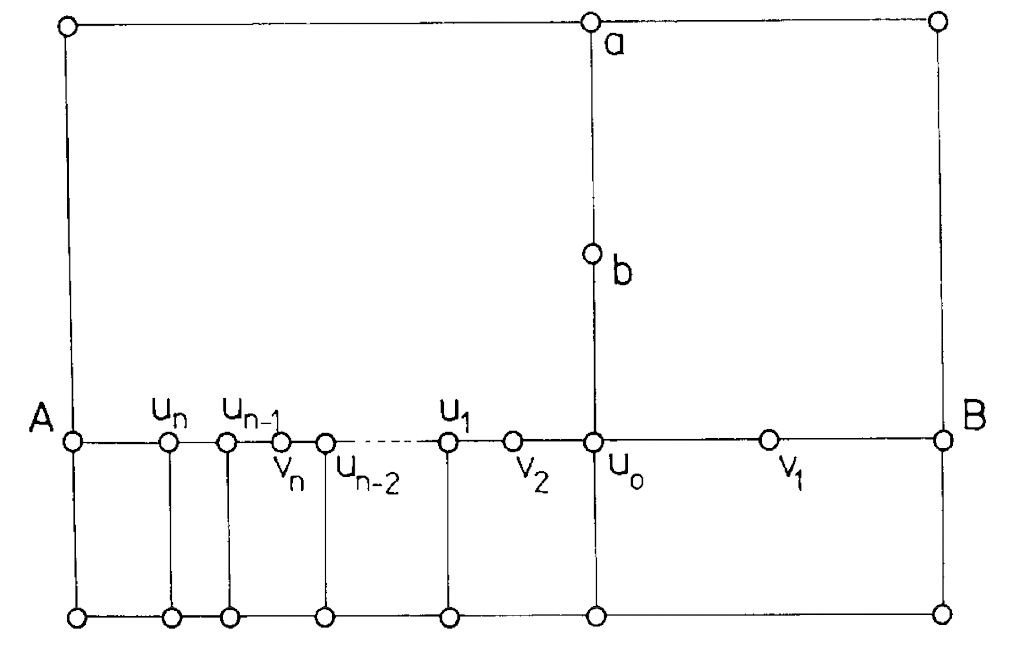
\includegraphics[width=\textwidth]{images/figure-11.png}
        \end{column}
    \end{columns}
\end{frame}

\begin{frame}[t]{Theorem \ref{thm:exp-cw} Proof}
    \begin{lemma*}
        In every weak realization, the edge \(\set{u_i, v_i}\) intersects 
        the edge \(\set{a,b}\) at least \(2^{i-1}\) times.
    \end{lemma*}
    \begin{columns}
        \begin{column}{0.5\textwidth}
            \begin{itemize}
                \item<2-> Induction start, \(i=1\): \(2^{1-0} = 1\) exactly one crossing of 
                \(\set{a,b}\) \(\checkmark\)
                \item<3-> Induction step: Let it hold for some \(i\).
                \item<4-> \(\set{u_{i+1}, v_{i+1}}\) is not allowed to cross \(\set{u_i, v_i}\).
                \item<5-> \(\Rightarrow\) it must make a turn around \(v_i\).
                \item<6-> Thus, it consists of two parts:
                \begin{enumerate}
                    \item<6-> from \(u_{i+1}\) to the turnpoint
                    \item<7-> from the turnpoint to \(v_{i+1}\)
                \end{enumerate}
            \end{itemize}
        \end{column}
        \begin{column}{0.5\textwidth}
            \includegraphics<1>[width=\textwidth]{images/figure-12.png}%
            \includegraphics<2>[width=\textwidth]{images/figure-13.png}%
            \includegraphics<3>[width=\textwidth]{images/figure-12.png}%
            \includegraphics<4>[width=\textwidth]{images/figure-14.png}%
            \includegraphics<5>[width=\textwidth]{images/figure-15.png}%
            \includegraphics<6>[width=\textwidth]{images/figure-16.png}%
            \includegraphics<7->[width=\textwidth]{images/figure-17.png}%
        \end{column}
    \end{columns}
\end{frame}

\begin{frame}[t]{Theorem \ref{thm:exp-cw} Proof}
    \begin{lemma*}
        In every weak realization, the edge \(\set{u_i, v_i}\) intersects 
        the edge \(\set{a,b}\) at least \(2^{i-1}\) times.
    \end{lemma*}
    \begin{columns}
        \begin{column}{0.5\textwidth}
            \begin{enumerate}
                \item \(u_{i+1}\) to turnpoint:
                \begin{itemize}
                    \item If we contract \(u_{i+1}\) and \(u_i\), it can be used as an edge joining \(u_i\) and \(v_i\).
                    \item<2-> \(\leadsto 2^{i-1}\) intersections
                \end{itemize}
                \item<3-> turnpoint to \(v_{i+1}\):
                \begin{itemize}
                    \item<3-> If we contract \(v_{i+1}\) and \(u_i\), it can be used as an edge joining \(u_i\) and \(v_i\).
                    \item<4-> \(\leadsto 2^{i-1}\) intersections
                \end{itemize}
            \end{enumerate}
            \begin{itemize}
                \item<5-> \(\Rightarrow\) \(2^{i-1} + 2^{i-1} = 2^i = 2^{(i+1) - 1}\) intersections \(\checkmark\)
                \item<6-> \(\Rightarrow c_w(5n + 13) \geq 2^{n - 1}\). \qed
            \end{itemize}
        \end{column}
        \begin{column}{0.5\textwidth}
            \includegraphics<1-2>[width=\textwidth]{images/figure-16.png}%
            \includegraphics<3-4>[width=\textwidth]{images/figure-17.png}%
            \includegraphics<5->[width=\textwidth]{images/figure-12.png}%
        \end{column}
    \end{columns}
\end{frame}

\begin{frame}{Exponential Representations}
    \begin{corollary}
        \(c_s(m) \geq 2^{\hat{c} m}\) for some constant \(\hat{c} > 0\).
        \label{cor:exp-cs}
    \end{corollary}
\end{frame}

\begin{frame}%[allowframebreaks] not needed, not that many references
    \frametitle{References}
    \printbibliography[heading=none]
\end{frame}

\end{document}
